%!TEX root = main.tex

\documentclass{vldb}
% \usepackage{paralist}
% Load basic packages
\usepackage{balance}  % to better equalize the last page
\usepackage{graphicx} % for EPS, load graphicx instead
\usepackage{url}      % llt: nicely formatted URLs
\usepackage{amsmath}
\usepackage{color}
\usepackage{cancel}
\usepackage{listings}
%\usepackage{wrapfig}
\usepackage{graphicx}
\usepackage{subcaption}
\setlength{\abovecaptionskip}{10pt plus 3pt minus 2pt}
% \usepackage[english]{babel}
\usepackage{booktabs}
\usepackage{graphicx}
% \usepackage{subfigure}
% \usepackage{caption}
% \usepackage[scriptsize, it, IT]{subfigure}
% \usepackage[font={scriptsize,it}]{caption}
% \usepackage{tikz}
%\usepackage{MinionPro}
% \usetikzlibrary{arrows,matrix,positioning}
\usepackage[ruled,vlined,algonl,boxed]{algorithm2e}
\usepackage{algorithmic}
\usepackage{wrapfig}
% \usepackage{framed}
\usepackage{enumitem}
\usepackage{xspace}
\usepackage{xcolor}
\usepackage{colortbl}
% \usepackage{newtxmath}
\usepackage[T1]{fontenc}

% llt: Define a global style for URLs, rather that the default one
\makeatletter
\def\url@leostyle{%
  \@ifundefined{selectfont}{\def\UrlFont{\sf}}{\def\UrlFont{\small\bf\ttfamily}}}
\makeatother
\urlstyle{leo}

\makeatletter
\def\@copyrightspace{\relax}
\makeatother

% To make various LaTeX processors do the right thing with page size.
\def\pprw{8.5in}
\def\pprh{11in}
\special{papersize=\pprw,\pprh}
\setlength{\paperwidth}{\pprw}
\setlength{\paperheight}{\pprh}
\setlength{\pdfpagewidth}{\pprw}
\setlength{\pdfpageheight}{\pprh}

\newtheorem{definition}{Definition}%[section]
\newtheorem{proposition}[definition]{Proposition}
\newtheorem{lemma}[definition]{Lemma}
\newtheorem{remark}[definition]{Remark}
\newtheorem{corollary}[definition]{Corollary}
\newtheorem{claim}[definition]{Claim}
\newtheorem{theorem}[definition]{Theorem}
\newtheorem{heuristic}[definition]{Heuristic}
\newtheorem{example}[definition]{Example}
%\newtheorem{proof}[definition]{Proof}
\newtheorem{dimension}{Dimension}
\newcounter{prob}
\newtheorem{problem}[prob]{Problem}
\newtheorem{conjecture}[definition]{Conjecture}
\newtheorem{reduction}[definition]{Reduction}
\newtheorem{property}[definition]{Property}
\newtheorem{axiom}[definition]{Axiom}
% 
% \tikzset{
%     %Define standard arrow tip
%     >=stealth',
%     %Define style for boxes
%     punkt/.style={
%            rectangle,
%            rounded corners,
%            draw=black, very thick,
%            text width=6.5em,
%            minimum height=2em,
%            text centered},
%     % Define arrow style
%     pil/.style={
%            ->,
%            thick,
%            shorten <=2pt,
%            shorten >=2pt,}
% }


% \setitemize{noitemsep,topsep=0pt,parsep=0pt,partopsep=0pt}

% \def\compactify{\itemsep=0pt \topsep=0pt \partopsep=0pt \parsep=0pt}
% \let\latexusecounter=\usecounter
% \newenvironment{CompactItemize}
%   {\def\usecounter{\latexusecounter}
%    \begin{itemize}[noitemsep,topsep=0pt,parsep=0pt,partopsep=0pt,leftmargin=*]}
%   {\end{itemize}\let\usecounter=\latexusecounter}
% \newenvironment{CompactEnumerate}
%   {\def\usecounter{\compactify\latexusecounter}
%    \begin{enumerate}[leftmargin=*]}
%   {\end{enumerate}\let\usecounter=\latexusecounter}


%%%  What is this?  Use enumitem instead
% 
% \newcommand{\squishlist}{
%    \begin{list}{$\bullet$}
%     { \setlength{\itemsep}{0pt}
%       \setlength{\parsep}{2pt}
%       \setlength{\topsep}{6pt}
%       \setlength{\partopsep}{0pt}
%       \leftmargin=25pt
% \rightmargin=0pt
% \labelsep=5pt
% \labelwidth=10pt
% \itemindent=0pt
% \listparindent=0pt
% \itemsep=\parsep
%     }
% }
% \newcommand{\squishend}{\end{list}}
% 
% 
% \newcommand{\squishframe}{\vspace{-6pt}
% \begin{framed} 
% \vspace{-6pt}}
% 
% \newcommand{\frameend}{\vspace{-6pt}
% \end{framed}
% \vspace{-6pt}}


% create a shortcut to typeset table headings
% \newcommand\tabhead[1]{\small\textbf{#1}}




% Make sure hyperref comes last of your loaded packages, 
% to give it a fighting chance of not being over-written, 
% since its job is to redefine many LaTeX commands.
\usepackage[pdftex]{hyperref}
\hypersetup{
  colorlinks=false,
  linkcolor=darkred,
  citecolor=darkgreen,
  urlcolor=darkblue
}
% \usepackage{cleveref} % After hyperref, listings



% Avoid widows and orphans
\widowpenalty=500
\clubpenalty=500

% % Aggressive figure placement
% \renewcommand{\topfraction}{0.9}
% \renewcommand{\bottomfraction}{0.8}
% \setcounter{topnumber}{2}
% \setcounter{bottomnumber}{2}
% \setcounter{totalnumber}{4}
% \setcounter{dbltopnumber}{2}
% \renewcommand{\dbltopfraction}{0.9}
% \renewcommand{\textfraction}{0.07}
% \renewcommand{\floatpagefraction}{0.7}
% \renewcommand{\dblfloatpagefraction}{0.7}

\definecolor{light-gray}{gray}{0.95}
\definecolor{mid-gray}{gray}{0.85}
\definecolor{darkred}{rgb}{0.7,0.25,0.25}
\definecolor{darkgreen}{rgb}{0.15,0.55,0.15}
\definecolor{darkblue}{rgb}{0.1,0.1,0.5}
\definecolor{blue}{rgb}{0.19,0.58,1}

\newcommand{\red}[1]{\textcolor{red}{#1}}
\newcommand{\green}[1]{\textcolor{green}{#1}}
\newcommand{\blue}[1]{\textcolor{blue}{#1}}
\newcommand{\orange}[1]{\textcolor{orange}{#1}}
\newcommand{\darkred}[1]{\textcolor{darkred}{#1}}
\newcommand{\darkgreen}[1]{\textcolor{darkgreen}{#1}}
\newcommand{\darkblue}[1]{\textcolor{darkblue}{#1}}





\newcommand{\papertext}[1]{#1}
\newcommand{\techreport}[1]{#1}

\newcommand{\alex}[1]{\noindent{\color{darkgreen}{Alexandra: #1}}}
\newcommand{\xlw}[1]{\noindent{\color{blue}{xl: #1}}}
\newcommand{\ewu}[1]{\noindent{\color{red}{EWu: #1}}}
\newcommand{\xxx}[1]{{\fontsize{13pt}{13pt}\selectfont\textcolor{red}{#1}}}
\newcommand{\codesize}{\fontsize{7}{8}}
\newcommand{\stitle}[1]{\vspace{0.5em}\noindent\textbf{#1}}
\newcommand{\calF}[0]{$\cal{F}$}

\newcommand{\ind}{\hspace{\algorithmicindent}}

% \newcommand{\deprecate}[1]{}
\newcommand{\deprecate}[1]{\noindent{\color{light-gray}{#1}}}

\newcommand{\prob}{{\sc Log-Corruption}\xspace}
\newcommand{\exact}{{\sc EXACTSOL}\xspace}
\newcommand{\qfix}{{\sc SingleQueryFix}\xspace}
\newcommand{\density}{{\sc DENSITY}\xspace}


\newcommand{\milpall}{\textsc{MILP-NAIVE}\xspace}
\newcommand{\milptuple}{\textsc{MILP-COMPL}\xspace}
\newcommand{\milptuplestopearly}{\textsc{MILP-COMPL-STOPEARLY}\xspace}
\newcommand{\milpadvtuple}{\textsc{MILP-ADV-TUPLE}\xspace}
\newcommand{\milpadvall}{\textsc{MILP-ADV-ALL}\xspace}
\newcommand{\heurstic}{\textsc{HEURISTIC}\xspace}

\pagenumbering{arabic}

%%Ensuring that equation labels remain normal size, even if we shrink the equation text
\makeatletter
\def\maketag@@@#1{\hbox{\m@th\normalfont\normalsize#1}}
\DeclareRobustCommand*\textsubscript[1]{%
          \@textsubscript{\selectfont#1}}
        \def\@textsubscript#1{%
          {\m@th\ensuremath{_{\mbox{\fontsize\sf@size\z@#1}}}}}
\makeatother

\newcommand{\sysname}{\textsc{QueryFix}}
\newcommand{\sys}{QFix\xspace}
\newcommand{\naive}{\sysname\textsubscript{basic}\xspace}
\newcommand{\tslice}{\sysname\textsubscript{ts}\xspace}
\newcommand{\qslice}{\sysname\textsubscript{qs}\xspace}
\newcommand{\aslice}{\sysname\textsubscript{as}\xspace}
\newcommand{\incremental}{\sysname\textsubscript{inc}\xspace}

% End of preamble. Here it comes the document.
\begin{document}

% for 
\title{{\sys}: Demonstrating error diagnosis in query histories}

\numberofauthors{3}
\author{
  \alignauthor Xiaolan Wang\\
    \affaddr{School of Computer Science}\\
    \affaddr{University of Massachusetts}\\
    \email{xlwang@cs.umass.edu}\\
  \alignauthor Alexandra Meliou\\
  \affaddr{School of Computer Science}\\
    \affaddr{University of Massachusetts}\\
    \email{ameli@cs.umass.edu}\\
  \alignauthor Eugene Wu\\
    \affaddr{Computer Science}\\
    \affaddr{Columbia University}\\
    \email{ewu@cs.columbia.edu}\\
}




{
\maketitle
\vspace*{-.5in}
}

\begin{abstract}

An increasing number of applications in all aspects of society rely on
data. Despite the long line of research in data cleaning and repairs,
data correctness has been an elusive goal. Errors in the data can be
extremely disruptive, and are detrimental to the effectiveness and
proper function of data-driven applications. Even when data is
cleaned, new errors can be introduced by applications and users who
interact with the data. Subsequent valid updates can obscure these
errors and propagate them through the dataset causing more
discrepancies. Any discovered errors tend to be corrected
superficially, on a case-by-case basis, further obscuring the true
underlying cause, and making detection of the remaining errors harder.

In this demo proposal, we outline the design of \sys, a {\it query-centric}
framework that derives explanations and repairs for discrepancies in 
relational data based on potential errors in the queries that operated on the data. 
This is a marked departure from traditional {\it data-centric} techniques that directly fix the data.
We then describe how users will use \sys in a demonstration scenario. 
Participants will be able to select from a number of 
transactional benchmarks, introduce errors into the queries that are executed,
and compare the fixes to the queries proposed by \sys as well as existing alternative algorithms
such as decision trees.

\end{abstract}

%!TEX root = ../main.tex

\section{Introduction}
\label{s:intro}

Data errors are a pervasive, expensive, and time consuming problem
that afflicts the vast majority of data-driven applications. For
example, errors in retail price data cost US consumers \$2.5 billion
each year~\cite{Fan2008}. In aggregate, studies estimate data errors
to cost the US economy more than \$600 billion per
year~\cite{eckerson2002}. Therefore, it is not surprising that a
significant fraction of time in data analysis --- up to
80\%~\cite{kandel2012} --- is devoted to cleaning and
wrangling~\cite{kandel2011wrangler} the data into a structured and
sufficiently clean form to use in downstream applications.

In response, both industry and academia has focused on data cleaning solutions to mitigate this problem.
ETL-type systems~\cite{systemt, informatica} focus on cleansing the data before it is loaded into the database
using a set of pre-defined rules; outlier and anomaly detection algorithms~\cite{} are used to identify errors
in the database after the data has been loaded; while recent approaches use downstream applications
such as interactive visualizations, application queries, or data-products to facilitate error detection and correction algorithms.
In each of these cases, the focus of error diagnosis and cleaning has been {\it data centric}, in the sense that
the process is meant to identify and directly fix data values.

These efforts have largely ignored an important source of data errors --- data modification {\it queries}.
Mistakes in such queries can introduce errors that spread throughout the database due to subsequent, possibly correct updates.
Consider the following salary management example:

% change example
%!TEX root = ../main.tex


\begin{figure*}[t]
    \begin{minipage}[t]{0.28\textwidth}
         \vspace{0pt} 
         \centering
        \begin{tabular}{llll}
            \multicolumn{4}{l}{\emph{Taxes}: $D_0$}\\
            \toprule
            \textbf{ID}  & \textbf{income}    & \textbf{owed} & \textbf{pay} \\
            \midrule
            $t_1$   & \$9500    & \$950		& \$8550 \\
            $t_2$   & \$90000   & \$22500 	& \$67500\\
            $t_3$   & \$86000   & \$21500	& \$64500\\
            $t_4$   & \$86500   & \$21625	& \$64875\\
            \bottomrule
            \\
        \end{tabular}
    \end{minipage}
    \begin{minipage}[t]{0.43\textwidth}
         \vspace{0pt} 
         \centering
        \begin{tabular}{|p{1ex}l|}
            \multicolumn{2}{l}{\emph{Query log}: $\mathcal{Q}$}\\
            % \toprule
            \hline
            
            $q_1$: & \texttt{\small UPDATE Taxes SET owed=income*0.3}\\
            	   & \texttt{\small WHERE income>=\color{red}{85700}}\\
            
            $q_2$: & \texttt{\small INSERT INTO Taxes}\\ 
                   & \texttt{\small VALUES (25, 85800, 21450)}\\
                   
            $q_3$: & \texttt{\small UPDATE Taxes SET pay=income-owed}\\ 
            \hline
            % \bottomrule
        \end{tabular}
    \end{minipage}
    \begin{minipage}[t]{0.28\textwidth}
         \vspace{0pt} 
         \centering
        \begin{tabular}{llll}
            \multicolumn{4}{l}{\emph{Taxes}: $D_4$}\\
            \toprule
            \textbf{ID}  & \textbf{income}    & \textbf{owed}  & \textbf{pay}\\
            \midrule
            $t_1$ & \$9500    & \$950		& \$8550\\
            $t_2$   & \$90000   & \$27000	& \$63000\\
            \rowcolor{mid-gray}
            $t_3$ & \$86000   & \color{red}{\$25800} & \color{red}{\$60200}\\
            \rowcolor{mid-gray}
            $t_4$	 & \$86500	  & \color{red}{\$25950}	& \color{red}{\$60550}\\
            $t_5$	 & \$87000	  & \$21750	& \$65250\\
            \bottomrule
        \end{tabular}
    \end{minipage}

    \caption{A recent change in tax rate brackets calls for a tax rate of 30\% for those with income above \$87500.  The accounting department issues query $q_1$ to implement the new policy, but the predicate of the WHERE clause condition transposed two digits of the income value.
\iffalse  
As a result, the owed amount of $t_3$ and $t_4$ were calculated incorrectly. 
This mistake is obscured by $q_2$ which insert a tuple with correct income and owed amount and later further propagated to additional filed(s) by query $q_3$ which calculates the pay check amount based on the corresponding income and (incorrect) owed values.
\fi
    % \alex{I am confused about what happened with this example.  The numbers in the figure don't match the description in Example 3.  This doesn't see to be used later (yet).  Before I fix it, I want to check whether there is a reason for the particular changes...}}\xlw{I changed this example for later optimization sec.6 and noise sec.7 handling explanation. There are two goals: 1. we will demonstrate why we need 2 iterations to reduce noise when we only encode tuples in the complaint set for efficiency; 2. we will show if how we detect and prune false positive complaint $t_5$ by constructing complaint-tuple bipartite graph and searching densest sub-graph. 
    }
    \label{fig:example}
\end{figure*}
%%!TEX root = ../main.tex


\begin{figure*}[t]
    \begin{minipage}[t]{0.28\textwidth}
         \vspace{0pt} 
         \centering
        \begin{tabular}{llll}
            \multicolumn{4}{l}{\emph{Taxes}: $D_0$}\\
            \toprule
            \textbf{ID}  & \textbf{income}    & \textbf{owed} & \textbf{pay} \\
            \midrule
            $t_1$   & \$9500    & \$950		& \$8550 \\
            $t_2$   & \$90000   & \$22500 	& \$67500\\
            $t_3$   & \$86000   & \$21500	& \$64500\\
            $t_4$   & \$86500   & \$21625	& \$64875\\
            \bottomrule
            \\
        \end{tabular}
    \end{minipage}
    \begin{minipage}[t]{0.43\textwidth}
         \vspace{0pt} 
         \centering
        \begin{tabular}{|p{1ex}l|}
            \multicolumn{2}{l}{\emph{Query log}: $\mathcal{Q}$}\\
            % \toprule
            \hline
            
            $q_1$: & \texttt{\small UPDATE Taxes SET owed=income*0.3}\\
            	   & \texttt{\small WHERE income>=\color{red}{85700}}\\
            
            $q_2$: & \texttt{\small INSERT INTO Taxes}\\ 
                   & \texttt{\small VALUES (25, 85800, 21450)}\\
                   
            $q_3$: & \texttt{\small UPDATE Taxes SET pay=income-owed}\\ 
            \hline
            % \bottomrule
        \end{tabular}
    \end{minipage}
    \begin{minipage}[t]{0.28\textwidth}
         \vspace{0pt} 
         \centering
        \begin{tabular}{llll}
            \multicolumn{4}{l}{\emph{Taxes}: $D_4$}\\
            \toprule
            \textbf{ID}  & \textbf{income}    & \textbf{owed}  & \textbf{pay}\\
            \midrule
            $t_1$ & \$9500    & \$950		& \$8550\\
            $t_2$   & \$90000   & \$27000	& \$63000\\
            \rowcolor{mid-gray}
            $t_3$ & \$86000   & \color{red}{\$25800} & \color{red}{\$60200}\\
            \rowcolor{mid-gray}
            $t_4$	 & \$86500	  & \color{red}{\$25950}	& \color{red}{\$60550}\\
            $t_5$	 & \$87000	  & \$21750	& \$65250\\
            \bottomrule
        \end{tabular}
    \end{minipage}

    \caption{A recent change in tax rate brackets calls for a tax rate of 30\% for those with income above \$87500.  The accounting department issues query $q_1$ to implement the new policy, but the predicate of the WHERE clause condition transposed two digits of the income value.
\iffalse  
As a result, the owed amount of $t_3$ and $t_4$ were calculated incorrectly. 
This mistake is obscured by $q_2$ which insert a tuple with correct income and owed amount and later further propagated to additional filed(s) by query $q_3$ which calculates the pay check amount based on the corresponding income and (incorrect) owed values.
\fi
    % \alex{I am confused about what happened with this example.  The numbers in the figure don't match the description in Example 3.  This doesn't see to be used later (yet).  Before I fix it, I want to check whether there is a reason for the particular changes...}}\xlw{I changed this example for later optimization sec.6 and noise sec.7 handling explanation. There are two goals: 1. we will demonstrate why we need 2 iterations to reduce noise when we only encode tuples in the complaint set for efficiency; 2. we will show if how we detect and prune false positive complaint $t_5$ by constructing complaint-tuple bipartite graph and searching densest sub-graph. 
    }
    \label{fig:example}
\end{figure*}

Although existing data-centric cleaning techniques may help identify and correct these reported errors directly, 
this is suboptimal because it treats the symptom --- the errors in the current database state --- rather than the anomalous
queries that are the underlying cause.  In practice, only a subset of the paystub errors will be reported, thus fixing
the reported errors on a case-by-case basis will likely obscure the root problem, making it more difficult to
find both the erroneous query and the other affected data.  
Furthermore, a data-centric approach must repair \emph{all errors} --- a non-repaired value such as the incorrect tax rate
may continue to introduce errors in the database through future queries 
(e.g., inserting incorrectly computed paychecks based on the still-incorrect tax rate).

\alex{Leaving this paragraph to Eugene.}
For these reasons, traditional data cleaning approaches may be helpful for finding errors in the data, but are
not designed to diagnose causes of the errors when they are rooted in incorrect queries.
There has been some work, but not directly for this problem.  
\ewu{fill in with related work}
Integrity constraints.
Certificate-based verification.
Structural sources of mistakes, but not identify the specific faulty query and how it is wrong.
In more restricted domains, data explanation finds predicates to exclude from queries, but only work for a single, simple  aggregation query.

Query-centric cleaning and repair is challenging because an error introduced by a query can be obscured by, or propagated throughout the database
by subsequent queries. This alludes to several factors that make even identifying problematic queries difficult:

\begin{enumerate}[leftmargin=*, topsep=0mm, itemsep=0mm]

  \item \textbf{Butterfly fffect: } 
  An error in even a single query can affect a large number of records, as documented in several real-world
  cases~\cite{Yates10, Grady13, sakalerrors}.  Even if a single record is incorrect,
  its value may be used as part of the \texttt{WHERE} or \texttt{SET} clauses of 
  subsequent valid queries that introduce additional errors that are seemingly unrelated.

  \item \textbf{Partial information:}  In most practical settings, we cannot assume that we can identify all
  errors in the database --- for example, not all employees will complain about their incorrect paystubs.  
  More likely, we only have access to a subset of the data errors, and must use them to extrapolate 
  the queries that affected a possibly larger set of data.  A diagnostic tool that can reduce
  the entire transaction log to the most likely candidate queries and propose fixes
  is needed to make this process manageable.


  \item \textbf{Multiple types of errors:} 
  An erroneous query can cause multiple types of data errors.  For example, a record that should not exist may have been accidentally inserted, or conversely a record that 
  should exist was unintentionally deleted.  Similarly, attribute values may be incorrectly updated,
  updated when they should not have been, or not updated when they should have.  
  Any combination of these error types may be present in the current state of the database,
  and although they may not be obviously related to each other, they must be addressed in a holistic manner.  

\end{enumerate}


In this demo proposal, we outline the design of \sys, a framework that derives explanations
and repairs for discrepancies in relational data based on potential errors in
the queries that operated on the data, and describe how users will use \sys
in a demonstration scenario. 
In contrast to existing approaches in data
cleaning that aim to detect and correct errors in the data directly, the goal
of \sys is to identify  the problematic queries that introduced errors into the
database. These diagnoses both \emph{explain} how errors were introduced to a
dataset, and also lead to the identification of additional discrepancies in
the data that would have otherwise remained undetected.
Participants will be able to 
select from a number of transactional benchmarks to generate a query workload,
introduce errors into the queries that are executed,
and compare the fixes to the queries proposed by \sys against existing alternative algorithms such as decision trees.



% Poor data quality is a hard and persistent problem.  It is estimated to cost the US economy more than \$600 billion
% per year~\cite{eckerson2002} and erroneous price data in retail databases
% alone cost the US consumers \$2.5 billion each year~\cite{Fan2008}. Although data
% cleaning tools can purge many errors from a dataset before downstream 
% applications use the data, databases are constantly changing as applications
% and users execute queries that modify the data.
% Mistakes in these queries can introduce errors that spread through the database
% due to subsequent update queries; 
% by the time errors are detected, it is difficult to trace those errors back to the 
% erroneous query and correct it.
% Identifying and correcting errors in the data directly is suboptimal: it treats the symptom,
% rather than the underlying cause. Fixing the manifested data errors on a
% case-by-case basis often obscures the root of the problem and other data that may have been
% affected. Therefore, traditional data cleaning approaches are not well-suited
% for this setting: While they provide general-purpose tools to identify and
% rectify anomalies in the data, they are not designed to diagnose the causes of
% errors that are rooted in erroneous updates.
% Some data cleaning systems try to identify structural sources of
% mistakes~\cite{wang2015}, but they are unable to trace the source of
% the mistakes to particular faulty queries.
% 
% While improving data quality and correcting data errors has been an important
% focus for data management research, handling new errors, introduced during
% regular database interactions, has received little attention. Most work in
% this direction focuses on \emph{guarding against} erroneous updates. For
% example, integrity constraints~\cite{Khoussainova2006} reject some improper
% updates, but only if the data falls outside rigid, predefined ranges.
% Certificate-based verification~\cite{Chen2011} is less rigid, but it is
% impractical and non-scalable as it requires users to answer challenge
% questions before allowing the updates, and it is not applicable to updates
% initiated by applications.





% \begin{example}[Wireless discount policies]\label{ex:telco}
% 
% A large US-based wireless provider offers company discounts as incentives for
% corporate customers. There are different types of discounts (flat, percentage,
% fee-based), and their details are specific to corporate agreements. The large
% number of policies and complexities in their rules frequently cause policies
% to be set incorrectly, leading to errors in the application of discounts to
% customers' accounts.
% 
% Customers who notice billing errors contact the provider, but the call centers
% do not have the capacity or ability to investigate the complaints deeply. The
% standard course of action is to correct billing mistakes on a case-by-case
% basis for each complaint. As a result, unreported errors remain in the
% database for a long time, or they never get corrected, and their cause becomes
% harder to trace as the source of the errors is obscured.\footnote{This is a real-life scenario, provided to us by a popular US-based wireless provider.}
% 
% \end{example}

% \begin{example}[Tax bracket adjustment]\label{ex:taxes}
%     
% Tax brackets, which determine tax rates for different income levels, are
% often adjusted. Accounting firms implement these changes to their
% databases by appropriately updating the tax rates of their customers. Mistakes
% in these update queries (e.g., Figure~\ref{fig:example}) result in errors in
% the tax rates and computed taxes. 
% 
% \end{example}
% 
% 
% In this application, data errors are typically reported to a
% customer service department, which does not have the resources nor the
% capability to investigate the errors more broadly. Instead, errors are
% resolved on a case-by-case basis. In practice, customer service only deals
% with a small portion of the actual errors. Once these errors are resolved,
% there will still be a large number of incorrect records that were not
% identified. The goal of \sys is to identify the query or queries that caused
% the errors, propose corrections to those queries, and use the modified queries
% to identify other errors.
% 
% Diagnosing data errors stemming from incorrect updates is fundamentally
% challenging: the search space of possible mistakes and fixes is large, and the
% amount of information (number of known errors) may be limited. The problem has
% the following important characteristics that render traditional data cleaning
% methods unsuitable:



% \begin{description}[leftmargin=*, topsep=0mm, itemsep=0mm]
%     
%     \item[Obscurity.] Detection of the resulting errors in the data often
%     leads to partial fixes that further complicate the eventual diagnosis and
%     resolution of the problem. For example, a transaction implementing a
%     change in the state tax law updated tax rates using the wrong rate,
%     affecting a large number of consumers. This causes a large number of
%     complaints to a call center, but each customer agent usually fixes each
%     problem individually, which ends up obscuring the source of the problem.
%     
%     \item[Large impact.] Erroneous queries cause errors at a large scale. The
%     potential impact of the errors is high, as manifested in several
%     real-world cases~\cite{Yates10, Grady13, sakalerrors}. Further, errors
%     that remain undetected for a significant amount of time can instigate
%     additional errors, even through valid updates. This increases both their
%     impact, and their obscurity.
%     
%     \item[Systemic errors.] The errors created by bad queries are
%     \emph{systemic}: they have common characteristics, as they share the same
%     cause. The link between the resulting data errors is the query that
%     created them; cleaning techniques should leverage this connection to
%     diagnose and fix the problem. Diagnosing the cause of the errors, will
%     achieve systematic fixes that will correct all relevant errors, even if
%     they have not been explicitly identified.
%    
% \end{description}
% 
% \sys addresses these challenges by analyzing the queries that operated on a
% dataset in an efficient and scalable manner. More concretely, we make the
% following contributions:


% The goal of this paper is to design effective query
% diagnosis techniques and identify possible fixes for query errors. We
% model the problem assuming a log of update workloads over a database,
% and a set of complaints that identify errors in the final database
% state. We organize our contributions as follows:

% \ewu{really like this organization}

% \ewu{add: special case optimizations for single query case.}


% \begin{itemize}[leftmargin=*, topsep=0mm, itemsep=0mm]      
%     \item We formalize the problem of diagnosing a set of errors using log
%     histories of updates that operated on the data. Given a set of 
%     \emph{complaints} as representations of data discrepancies in the current
%     state of a dataset, \sys identifies the queries in the log that require the  minimal
%     amount of changes that would resolve all of the complaints (Section~\ref{sec:abstractions}).
%       
%     \item We provide an exact error-diagnosis solution through a non-trivial
%     transformation of the problem to a mixed integer linear program (MILP) that
%     encodes the data provenance of the erroneous tuples. Our approach employs state-of-the-art MILP solvers to identify
%     optimal diagnoses that are guaranteed to resolve all complaints without introducing new errors to the data
%     (Section~\ref{sec:sol}).
%     
%     \item We present several optimizations to our basic diagnostic
%     method, which reduce the problem size without affecting the
%     quality of the produced solutions. Further, we propose an
%     incremental repair method that targets the cases where the log
%     contains a single corrupted query (or the search focuses on a
%     single repair). This incremental analysis of the log allows us to
%     scale to very large datasets and large query logs. Further, we
%     show that our optimization techniques have the additional
%     advantage of tolerating incomplete information, such as unreported
%     errors (Section~\ref{sec:opt}).
% 
%     
%     % \item We extend our framework to also handle false positives: complaints
%     % that mistakenly identify data as erroneous. We define the notion of
%     % complaint \emph{density}, which is a query-driven measure of closeness of
%     % a complaint to other complaints. The main intuition of our approach is
%     % that complaints of low density are likely false positives and thus can be
%     % safely ignored (Section~\ref{???}).
%     
%     \item We experimentally evaluate the effectiveness and efficiency of our
%     methods against real-world and synthetic datasets and query logs. 
%     (Section~\ref{sec:experiments}). 
% \end{itemize}

\section{The {\large\textbf{\sys}} Architecture}

\begin{figure}[h]
    \centering
        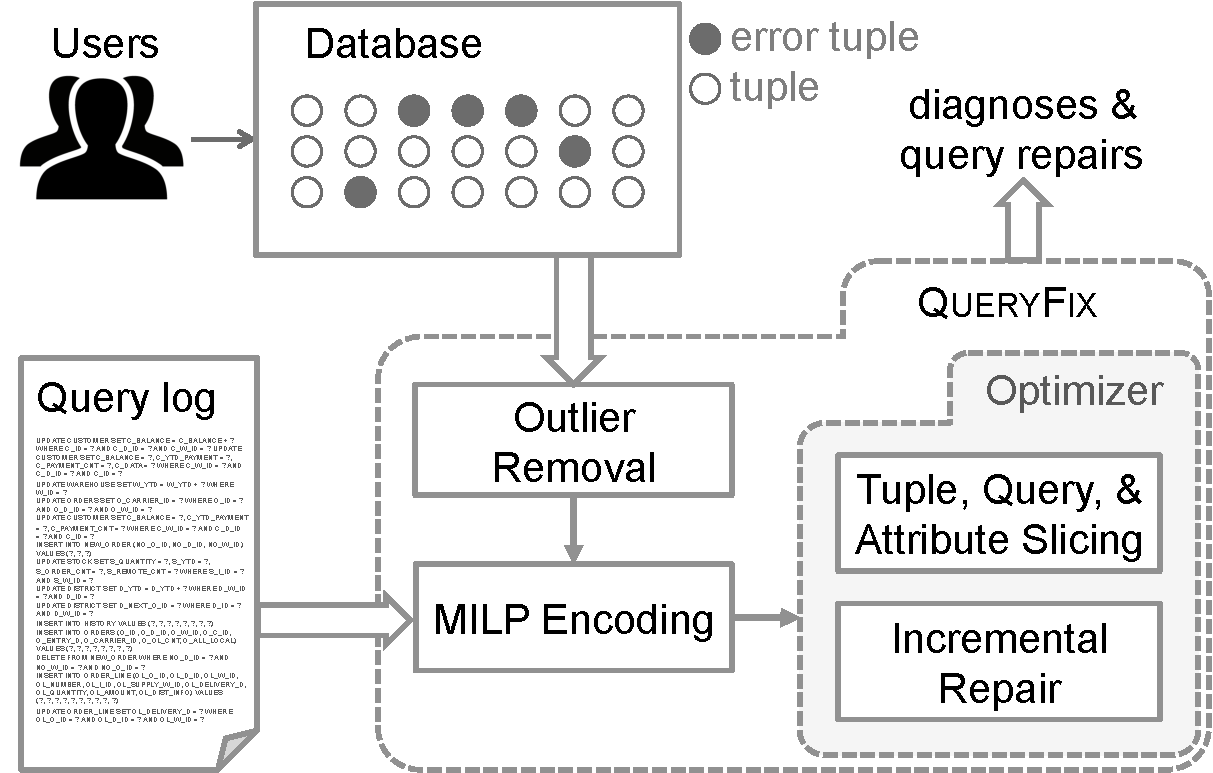
\includegraphics[scale=0.3]{figures/architecture}
    %\caption{\sys processes data anomalies in the form of complaints and analyzes logged query histories to identify the causes of error. 
    %In the heart of the system, the diagnosis problem is translated into a mixed integer linear program, and optimization modules ensure that the MILP programs can be evaluated efficiently.}
    \caption{\sys architecture diagram}
    \label{fig:architecture}
\end{figure}


Figure~\ref{fig:architecture} shows \sys's major components.  \sys takes as input 
a query log containing UPDATE, INSERT and DELETE queries, the database, along with a
set of identified data errors (called {\it complaints}).  These complaints are pairs
of tuple id of tuples that are wrong, along with an estimate of their correct values 
(e.g., $21500$ as tuple $t_3$'s tax value in Example~\ref{ex:telco}).
\sys uses this information to trace the causes of the errors and output the most likely set of 
queries in the log ({\it diagnoses}), along with proposed {\it repairs} of these queries.

To achieve this, \sys first performs an optional outlier removal step to deal with potential
false positives in the complaints.  Then the {\it MILP Encoding} component transforms the
query diagnosis problem into a Mixed Integer Linear Program (MILP) that is further optimized
through slicing and incremental repair techniques, before being sent
to an industrial MILP solver.  The output of the solver constitutes solutions to the query diagnosis
problem.

%!TEX root = ../main.tex

\section{Modeling abstractions}
\label{sec:abstractions}

In this section, we introduce a running example inspired from the use-case of
Example~\ref{ex:taxes}, and describe the model abstractions that we use to
formalize the diagnosis problem.


% \ewu{Add text to say false positive complaints are an orthogonal problem.}

%!TEX root = ../main.tex


\begin{figure*}[t]
    \begin{minipage}[t]{0.28\textwidth}
         \vspace{0pt} 
         \centering
        \begin{tabular}{llll}
            \multicolumn{4}{l}{\emph{Taxes}: $D_0$}\\
            \toprule
            \textbf{ID}  & \textbf{rate}  & \textbf{income}    & \textbf{owed}\\
            \midrule
            $t_1$   & 10    & \$9500    & \$950\\
            $t_2$   & 25    & \$90000   & \$22500\\
            $t_3$   & 25    & \$86000   & \$21500\\
            \bottomrule
            \\
        \end{tabular}
    \end{minipage}
    \begin{minipage}[t]{0.43\textwidth}
         \vspace{0pt} 
         \centering
        \begin{tabular}{|p{1ex}l|}
            \multicolumn{2}{l}{\emph{Query log}: $\mathcal{Q}$}\\
            % \toprule
            \hline
            $q_1$: & \texttt{\small UPDATE Taxes SET rate = 30}\\
                   & \texttt{\small WHERE income >= \color{red}{85700}} \\
            
            $q_2$: & \texttt{\small UPDATE Taxes SET owed = income*rate/100}\\
            
            $q_3$: & \texttt{\small INSERT INTO Taxes}\\ 
                   & \texttt{\small VALUES (4, 25, 86500, 21625)}\\
            \hline
            % \bottomrule
        \end{tabular}
    \end{minipage}
    \begin{minipage}[t]{0.28\textwidth}
         \vspace{0pt} 
         \centering
        \begin{tabular}{llll}
            \multicolumn{4}{l}{\emph{Taxes}: $D_3$}\\
            \toprule
            \textbf{ID}  & \textbf{rate}  & \textbf{income}    & \textbf{owed}\\
            \midrule
            $t_1$   & 10    & \$9500    & \$950\\
            $t_2$   & 30    & \$90000   & \$27000\\
            \rowcolor{mid-gray}
            $t_3$   & \color{red}{30}    & \$86000   & \color{red}{\$25800}\\
            $t_4$   & 25    & \$86500   & \$21625\\
            \bottomrule
        \end{tabular}
    \end{minipage}

    \caption{A recent change in tax rate brackets calls for a tax rate of 30\% for those with income above \$87500.  The accounting department issues query $q_1$ to implement the new policy, but the predicate of the WHERE clause condition transposed two digits of the income value.  As a result, the tax rate of $t_3$ was increased incorrectly.  Query $q_2$ that calculates the amount owed based on the corresponding tax rate and income propagates the error.  The mistake is further obscured by query $q_3$, which inserts a tuple with similar income and the correct tax rate.}
    \label{fig:example}
\end{figure*}

\begin{example}\label{ex:taxes2}
    
Figure~\ref{fig:example} demonstrates an example tax bracket adjustment in the
spirit of Example~\ref{ex:taxes}. The adjustment sets the tax rate to 30\% for
income levels above \$87,500, and is implemented by query $q_1$. A digit
transposition mistake in the query, results in an incorrect tax rate for tuples
$t_3$ and $t_4$. Query $q_2$ that calculates the amount owed based on the corresponding
tax rate and income propagates the error to other fields. The mistake is
further obscured by query $q_3$, which inserts a tuple with slightly higher
income than $t_3$ and $t_4$ and the correct (lower) tax rate.

\end{example}
% 
While traditional data cleaning techniques seek to identify and correct the
erroneous values in the table \emph{Taxes} directly, our goal is to diagnose
the problem, and understand the reasons for these errors. In this case, the
reason for the data errors is the incorrect predicate value in query $q_1$.

In this paper, we assume that we know \emph{some} errors in the dataset, and
that these errors were caused by erroneous updates. The errors may be
obtained in different ways: traditional data cleaning tools may identify
discrepancies in the data (e.g., a tuple with lower income has higher tax
rate), or errors can be reported directly from users (e.g., customers
reporting discrepancies to customer service). \emph{Our goal is not to correct
the errors directly in the data, but to analyze them as a ``symptom'' and provide a
diagnosis.} The diagnosis can produce a targeted treatment: knowing how the
errors were introduced guides the proper way to trace and resolve them.


%!TEX root=../main.tex

\begin{figure}[t]
\centering
{\small
\begin{tabular}{ll}
    \toprule
    \textbf{Notation} & \textbf{Description}\\
    \midrule
    $\mathcal{Q}$& The sequence of executed update queries (log)\\ 
             & $\mathcal{Q}=\{q_1, \dots, q_n\}$ \\
    $D_0$    & Initial database state at beginning of log\\
    $D_n$    & End database state (current) $D_n=\mathcal{Q}(D_0)$\\
    $D_i$    & Database state after query $q_i$: $D_i=q_i(\dots q_1(D_0))$\\
    $c: t\mapsto t^*$ & Complaint: $\mathcal{T}_c(D) = (D_n\setminus\{t\})\cup\{t^*\}$\\
    $\mathcal{C}$ & Complaint set $\mathcal{C}=\{c_1,\dots,c_k\}$\\
    $\mathcal{Q}^*$& Diagnosis or log repair\\
    $d(\mathcal{Q}, \mathcal{Q}^*)$ & Distance functions between two query logs\\
    \bottomrule
\end{tabular}
}
\caption{Summary of notations used in the paper. \alex{to update once finalized}}
\label{tbl:notation}
\end{figure}

\subsection{Error modeling}
\label{sec:model}

In our setting, the diagnoses are associated with errors in the queries that
operated on the data. In Example~\ref{ex:taxes2}, the errors in the dataset
are due to the digit transposition mistake in the WHERE clause predicate of
query $q_1$. Our goal is to infer the errors in a log of queries
automatically, given a set of incorrect values in the data. We proceed to
describe our modeling abstractions for data, queries, and errors, and how we
use them to define the diagnosis problem.

\subsubsection*{Data and query models}
\label{sec:models}

\noindent
\emph{Query log ($\mathcal{Q}$):}
We define a query log as an ordered sequence of \texttt{UPDATE}, \texttt{INSERT}, and
\texttt{DELETE} queries $\mathcal{Q}=\{q_1,\dots,q_n\}$, that have
operated on a database $D$. In the rest of the paper, we use the term
\emph{update queries}, or just \emph{queries}, to refer to any of the queries in $\mathcal(Q)$,
including insertion and deletion queries.

\smallskip
\noindent
\emph{Query ($q_i$):} We model each query as a function over a
database $D$, resulting in a new database $D'$. For \texttt{INSERT}
queries, $D'=q(D)=D\cup\{t_{new}\}$.
We model \texttt{UPDATE} and \texttt{DELETE} queries as follows:  
\begin{align*}
    D'=q(D)= &\{\mu_{q}(t)\;|\;t\in D, \sigma_{q}(t)\}%\\
    % &
    \cup\{t\;|\;t\in D, \neg\sigma_{q}(t)\}%\\
    % &\cup\{t_{new}\;|\;q\in\texttt{INSERT}\}
\end{align*}
% 
In this definition, the modifier function $\mu_q(t)$ represents the query's update equations, and it transforms a tuple by either deleting it ($\mu_q(t)=\bot$) or changing the values of some of its attributes.
The conditional function $\sigma_q(t)$ is a boolean function that represents the query's condition predicates.  In the example of Figure~\ref{fig:example}:
\begin{align*}
    &\mu_{q_1}(t)=(30, t.income, t.owed)\\
    &\sigma_{q_1}(t)=(t.income\ge 85700)\\
    &\mu_{q_2}(t)=(t.rate, t.income, \frac{t.income\cdot t.rate}{100})\\
    &\sigma_{q_2}(t)=\texttt{true}
\end{align*} 
% 
% As an insertion query, $q_3$ has $\sigma_{q_3}(t)=\texttt{false}$ and $t_{new}=(25, 85800, 21450)$.
% \ewu{why does it return false?  should it only be true if input is $\bot$?}


\smallskip
\noindent
\emph{Database state ($D_i$):}
We use $D_i$ to represent the state of a database $D$ after the application of
queries $q_1$ through $q_i$ from the log $\mathcal{Q}$. $D_0$ represents the
original database state, and $D_n$ the final, or current, database state. Out
of all the states, the system only maintains $D_0$ and $D_n$. In practice,
$D_0$ can be a checkpoint: a state of the database that we assume is correct;
we cannot diagnose errors before this state. The intermediate states can be
derived by executing the log: $D_i=q_i(q_{i-1}(\dots q_1(D_0)))$. We also
write $D_n=\mathcal{Q}(D_0)$ to denote that the final database state $D_n$ can
be derived by applying the sequence of queries in the log to the original
database state $D_0$.

\smallskip
\noindent
\emph{True database state ($D_i^*$):}
Queries in $\mathcal{Q}$ are possibly erroneous, introducing errors in the
data. There exists a sequence of \emph{true} database states $\{D_0^*,
D_1^*\dots, D_n^*\}$, with $D_0^*=D_0$, representing the database states that
would have occurred if there had been no errors in the queries.
The true database states are unknown; our goal is to find and correct the errors in $\mathcal{Q}$ and retrieve the correct database state $D_n^*$.

For ease of exposition, in the remainder of the paper we assume that the
database contains a single relation with attributes $A_i,\ldots,A_m$,
but the single table is not a requirement in our framework.


\subsubsection*{Error models}

Following the terminology in Examples~\ref{ex:telco}
and~\ref{ex:taxes}, we model a set of identified or user-reported
data errors as \emph{complaints}. A complaint corresponds to a
particular tuple in the final database state $D_n^*$, and identifies
that tuple's correct value assignment. We formally define complaints
below:

\begin{definition}[Complaint]
    A complaint $c$ is a mapping between two tuples: $c: t\mapsto t^*$, such that $t$ and $t^*$ have the same schema, $t\in D_n\cup\{\bot\}$, and $t\neq t^*$. A complaint defines a
    transformation $\mathcal{T}_c$ on a database state $D$: $\mathcal{T}_c(D)
    = (D\setminus\{t\})\cup\{t^*\}$.
\end{definition}

In the example of Figure~\ref{fig:example}, two complaints are reported on the final database state $D_3$: 
$c_1: t_3\mapsto t_3^*$ and
$c_2: t_4\mapsto t_4^*$, where $t_3^*=(25,86000,21500)$
and $t_4^*=(25,86500,21625)$.  For both these cases, each complaint denotes a value correction for a tuple in $D_3$.  Complaints can also model the addition or removal of tuples: $c: \bot\mapsto t^*$ means that $t^*$ should be added to the database, whereas $c: t\mapsto \bot$
means that $t$ should be removed from the database.


\smallskip
\noindent
\emph{Complaint set ($\mathcal{C}$):}
We use $\mathcal{C}$ to denote the set of all known complaints
$\mathcal{C}=\{c_1,\dots,c_k\}$, and we call it the \emph{complaint set}.
Each complaint in $\mathcal{C}$ represents a transformation (addition,
deletion, or modification) of a tuple in $D_n$. We assume that the
complaint set is consistent, i.e., there are no two complaints that
propose different transformations to the same tuple $t\in D_n$.
Applying all these transformations to $D_n$ results in a new database
instance
$D_n'=\mathcal{T}_{c_1}(\mathcal{T}_{c_2}(\dots\mathcal{T}_{c_k}(D_n)))$.\footnote{Since
the complaint set is consistent, it is easy to see that the order of
transformations is inconsequential.} $\mathcal{C}$ is \emph{complete}
if it contains a complaint for each error in $D_n$. In that case,
$D_n'=D_n^*$. In our work, we do not assume that the complaint set is
complete, but, as is more common in practice, we only know a subset of
the errors (incomplete complaint set). Further, we focus our analysis
on \emph{valid} complaints; we briefly discuss dealing with invalid
complaints (complaints identifying a correct value as an error) in
Section~\ref{sec:noise}, but these techniques are beyond the scope of this paper.

\smallskip
\noindent
\emph{Log repair ($\mathcal{Q}^*$):}
The goal of our framework is to derive a diagnosis as a log repair
$\mathcal{Q}^*=\{q_1^*,\dots, q_n^*\}$, such that
$\mathcal{Q}^*(D_0)=D_n^*$. In this work, we focus on errors produced
by incorrect parameters in queries, so our repairs focus on altering
query constants rather than query structure. Therefore, for each query
$q_i^*\in\mathcal{Q}^*$, $q_i^*$ has the same structure as $q_i$
(e.g., the same number of predicates and the same variables in the \texttt{WHERE} clause), 
but possibly different parameters. For example, a good log repair for the
example of Figure~\ref{fig:example} is
$\mathcal{Q}^*=\{q_1^*,q_2,q_3\}$, where $q_1^*$=\texttt{UPDATE Taxes
SET rate = 30 WHERE income >= 87500}.


\subsubsection*{Problem definition}

We now formalize the problem definition for diagnosing data
errors using query logs. A diagnosis is a log repair
$\mathcal{Q}^*$ that resolves all complaints in the set $\mathcal{C}$
and leads to a correct database state $D_n^*$.

\begin{definition}[Optimal diagnosis]\label{def:problem}
    Given database states $D_0$ and $D_n$, a query log $\mathcal{Q}$ such that $\mathcal{Q}(D_0)=D_n$, a set of complaints $\mathcal{C}$ on $D_n$,  and a distance function $d$, the optimal diagnosis is a log repair $\mathcal{Q}^*$, such that:
    \begin{itemize}[itemsep=0pt, parsep=0pt]
        \item $\mathcal{Q}^*(D_0)=D_n^*$, where $D_n^*$ has no errors
        \item $d(\mathcal{Q}, \mathcal{Q}^*)$ is minimized
    \end{itemize}
\end{definition}

More informally, we seek the minimum changes to the log $\mathcal{Q}$
that would result in a clean database state $D_n^*$. Obviously, a
challenge is that $D_n^*$ is unknown, unless we know that the
complaint set is complete. 

In Section~\ref{sec:sol}, we describe our basic method \naive, which
uses a constraint programming formulation that expresses this
diagnosis problem as a mixed integer linear program (MILP). We justify
using this constraint formulation as opposed to methods, such as
classification, that can analyze one query at a time in
Section~\ref{sec:heuristic}. We show that the latter, heuristic
approach is flawed, and one needs to encode the constraints in the
entire log. In Section~\ref{sec:opt}, we present several optimization
techniques that extend our basic method, allowing \sys to (1)~handle
cases of incomplete information (incomplete complaint set), and
(2)~scale to large data and log sizes. Specifically, our incremental
repair method (\incremental, Section~\ref{sec:incremental}), can
handle $10\times$ compared to the basic MILP approach.


% \begin{figure}[t]
% \centering
% 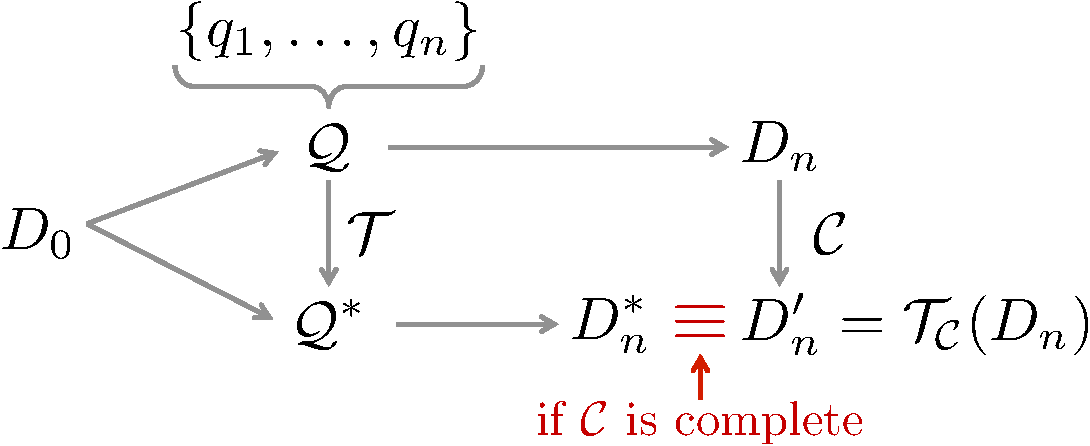
\includegraphics[width = 0.75\columnwidth]{figures/probtransform}
% \caption{Graphical depiction of the diagnosis problem in our \sys framework.  $D_0$, $D_n$, $\mathcal{Q}$, and $\mathcal{C}$ are given, and \sys uses them to derive the log repair $\mathcal{Q}^*$.
% \alex{not sure if this figure is actually useful.}}
% \label{f:probtransform} 
% \end{figure}


% \deprecate{
% \subsection{Naive Formulation}
% 
% The most general version of the problem
% (depicted in Figure~\ref{f:probtransform}) is to find a sequence of
% transformations $T$ that insert, delete, and/or modify queries in $Q_{seq}$ 
% such that the resulting sequence, $Q'_{seq} = T(Q_{seq})$, resolves the user's complaint set. 
% 
% However this problem is ill-defined because there exist an unbounded set of transformations that
% can resolve the user's complaint set.  A naive solution is to append to the query log a statement
% that deletes all the records in the database, followed by a query that insert all of the correct records.
% Unfortunately this naive solution does not help explain the complaints in any way!
% 
% \subsection{Constraints}
% 
% For this reason, we constrain the set of possible transformations $\mathcal{T}$ to the following:
% 
% \begin{itemize}
% \item delete query
% \item modify insert statement constants
% \item modify constants in WHERE clause
% \end{itemize}
% 
% Our transformations don't include adding new queries, synthesizing arbitrary queries, or modifying the
% number of clauses in a WHERE condition.  We apply these restrictions because we believe it is more likely
% for the user to mis-type a constant value as opposed to having an error in the query structure.
% 
% Futhermore we define a distance metric between two query logs in order to evaluate
% the qulatiy of a transformation.
% \xxx{define $\mathcal{T}$ here.}
% 
% 
% 
% \subsection{Problem Statements}
% 
% In this paper, we present three variants of this problem.
% 
% \begin{problem}[Prob-Complete]\label{prob:complete}
% Given $C = P_{D_n, D^*_n}$, $Q_{seq}$, and the sequence of database states $D_0,\ldots,D_n$, 
% identify a sequence of transformations $T$ such that:
% \begin{itemize}
% \item $T(Q_{seq})(D_0) = C(D_n)$
% \item $|T| = 1$
% \item $T$ metric is minimized
% \end{itemize}
% \end{problem}
% 
% This variation of the problme relaxes the constraint that the complaint set must be complete, and allows
% for both false positives as well as false negatives.  The goal is the same, however the constraints are relaxed:
% 
% \begin{problem}[Prob-Incomplete]\label{prob:incomplete}
% Given $C$ where $acc_C < 1$, $Q_{seq}$, and the sequence of database states $D_0,\ldots,D_n$, 
% identify a sequence of transformations $T$ such that:
% \begin{itemize}
% \item $T(Q_{seq})(D_0) = D^*_n$
% \item $T$ metric is minimized.
% \item $|T| = 1$
% \end{itemize}
% \end{problem}
% 
% Finally, we extend the problem to allow transformations with one or more operations.
% 
% \begin{problem}[Prob-MultiQ]\label{prob:multi}
% Given $C$ where $acc_C < 1$, $Q_{seq}$, and the sequence of database states $D_0,\ldots,D_n$, 
% identify a sequence of transformations $T$ such that:
% \begin{itemize}
% \item $T(Q_{seq})(D_0) = D^*_n$
% \item $T$ metric is minimized.
% \end{itemize}
% \end{problem}
% 
% 
% 
% 
% \subsection{A Naive Approach}
% 
% \begin{itemize}
% \item roll back complaints to penultimate state using algebraic expressions 
% \item perturb each expression in query until the query result matches correct state
% \item if an expression cannot be found, iterate
% \end{itemize}
% 
% 
% Not clear how to roll back complaints
% 
% Ways to perturb query expressions is unbounded
% 
% }
\section{Demonstration Outline}
\label{sec:demo}

In this section, we detail the proposed demonstration. The objective
of this demonstration is to show how \sys can quickly and accurately detect 
and propose fixes to errors in a query log, and compare its results to alternatives
that use existing techniques.


\begin{figure}[h]
\centering
  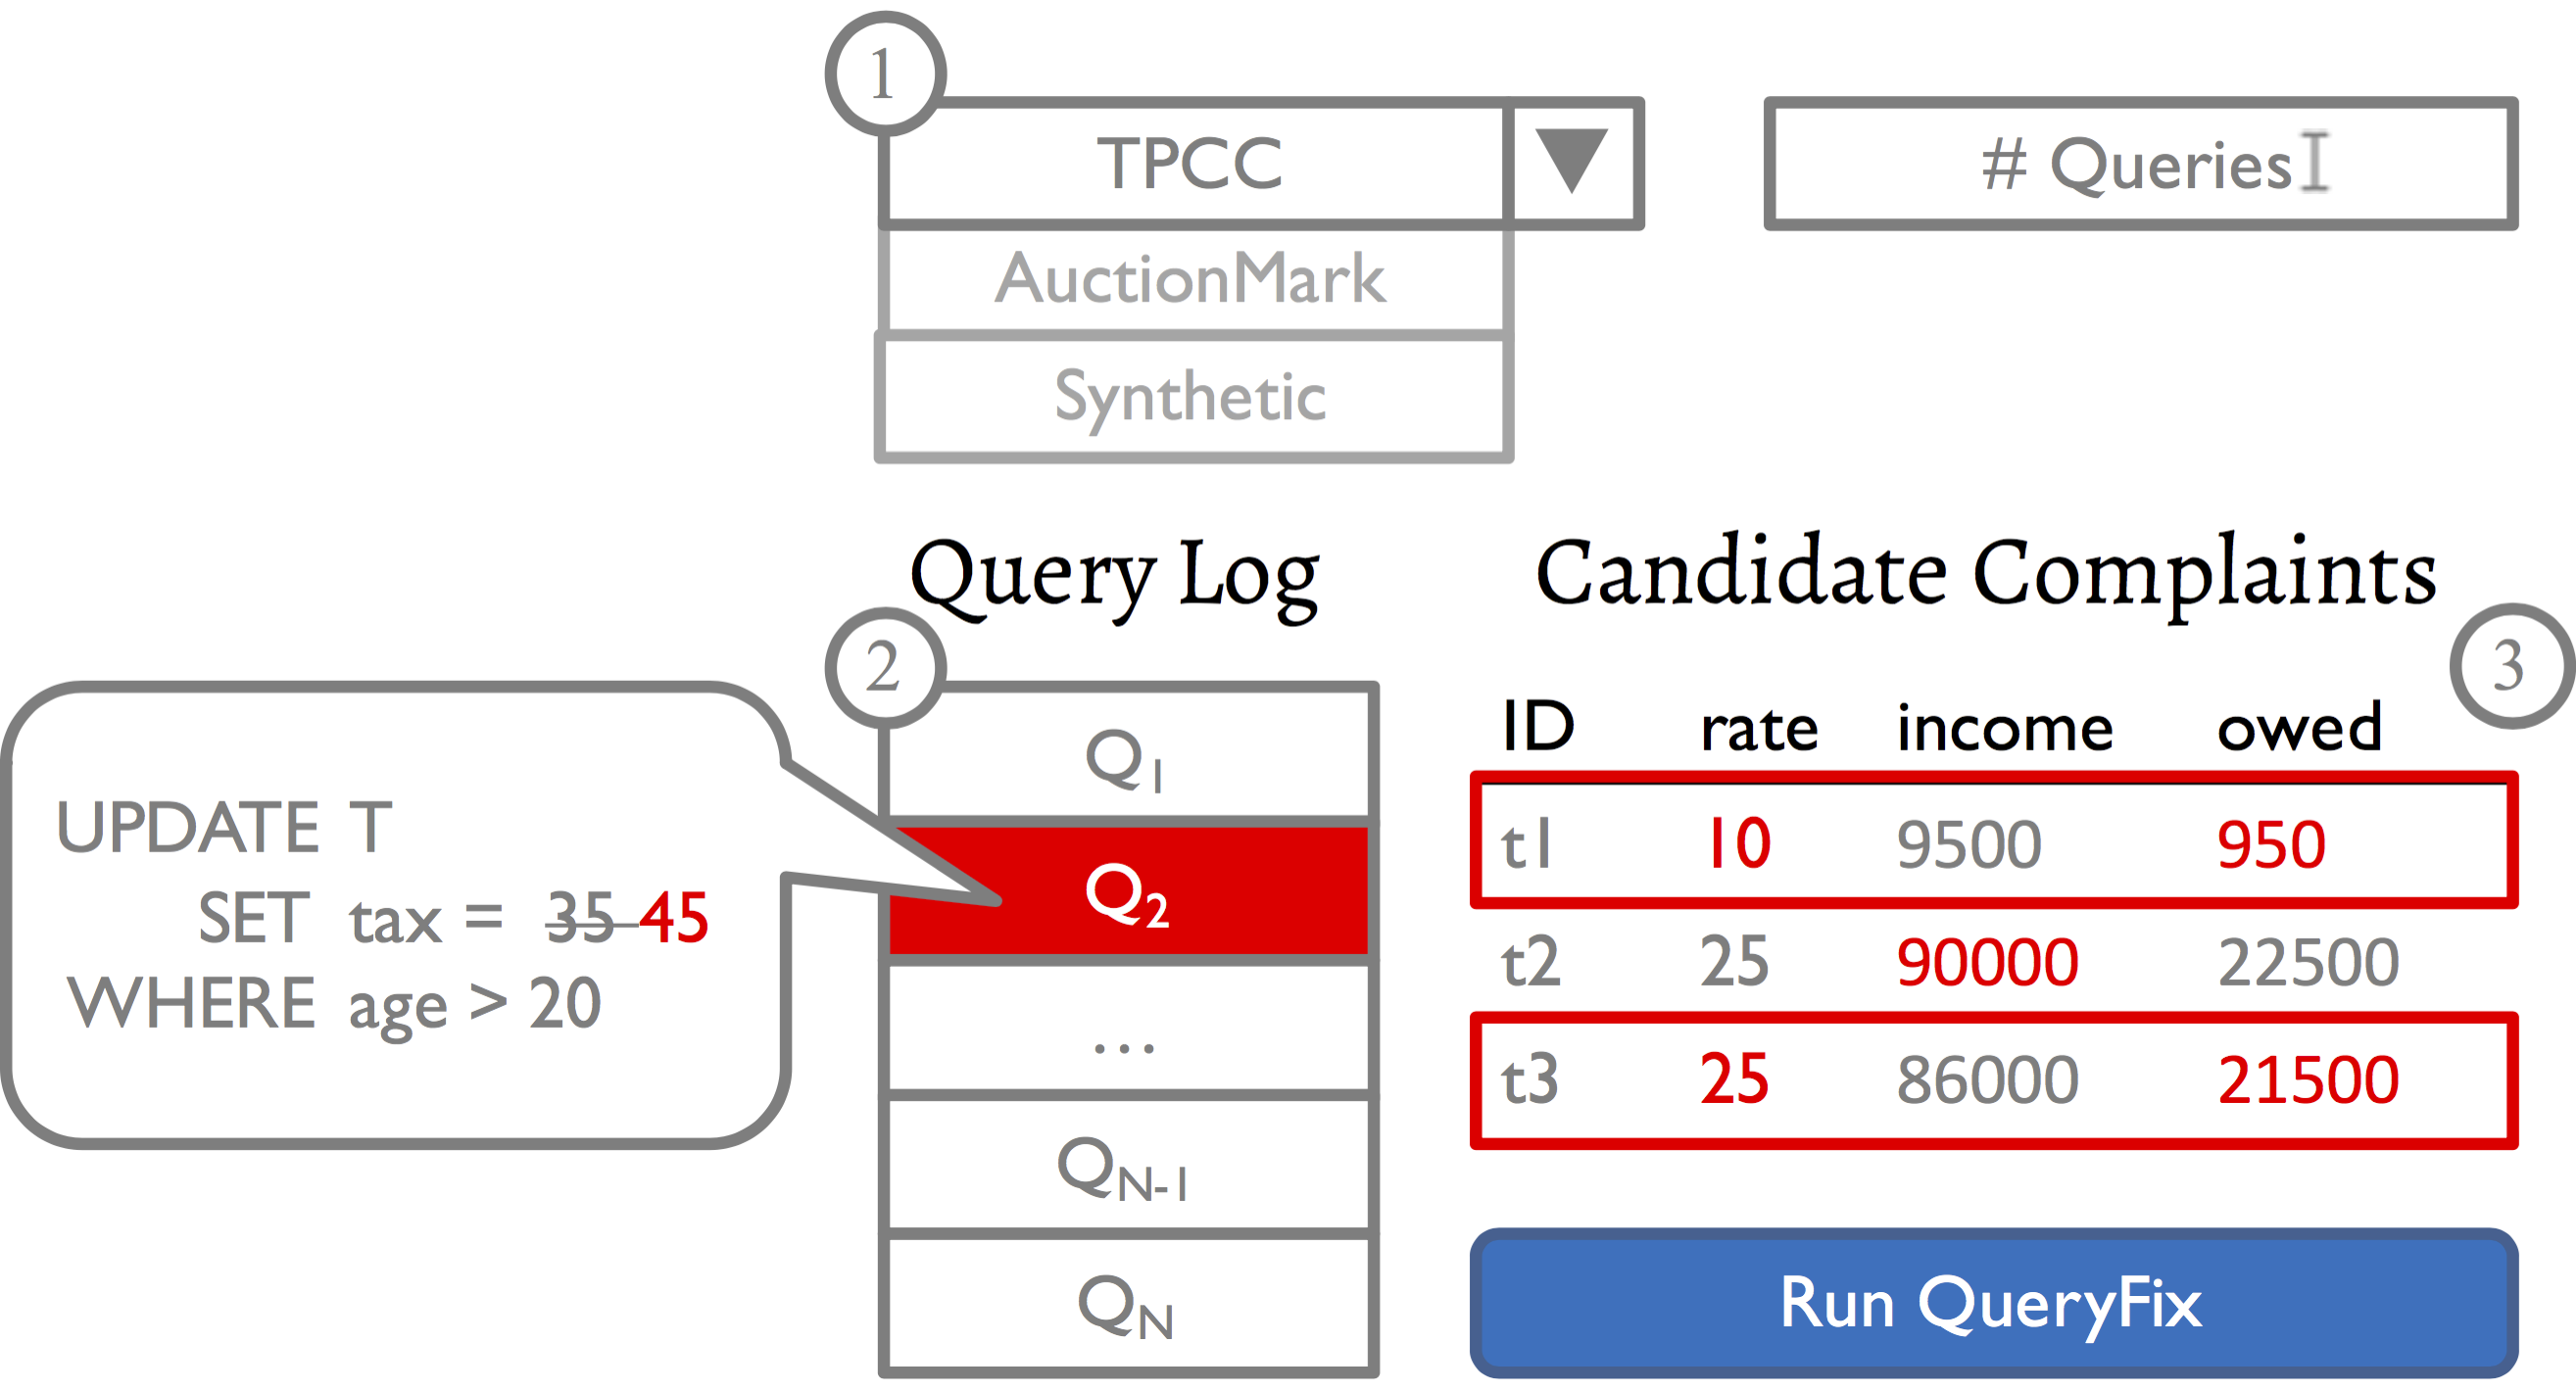
\includegraphics[width = .75\columnwidth]{figures/demo1}
  \caption{Users select and introduce errors to benchmark query workloads.}
  \label{f:demo1} 
\end{figure}

Figures~\ref{f:demo1} and~\ref{f:demo2} show screenshots of the initial and results pages.
Each step is annotated with a circled number, which we detail below.

\noindent {\bf Step 1 (Select Dataset):} Participants may first choose from a dropdown menu containing
a number of transaction workload generators from the benchmarks in OLTPBench~\cite{oltpbench}.
Since most transactional benchmarks focus on point update queries, we additionally include a 
synthetic workload generator that includes range updates, as well as insert and delete queries.
The text box on the right side allows users to additionally specify the number of queries to generate
in the workload.  

\noindent {\bf Step 2 (Corrupt the Query Log):} 
Once the workload generator is specified, the Query Log component of the interface
renders a scrollable list containing all of the queries.  When users select a query in the log,
the interface shows the query in an editable popup so that users can edit the queries, thus introducing errors
into the workload.  For example, in the figure, the user has edited query $Q_2$ by changing the \texttt{SET}
clause from $tax = 35$ to $tax = 45$.

\noindent {\bf Step 3:} The modified query cause the state of the database at the end of the workload
to differ from the result of the original workload.  The candidate complaints table lists the tuples
that are different and highlights the attribute values in those tuples as red text.  For instance,
$t_1.rate$ and $t_1.owed$ are both errors introduced by the modified query.  Users can select individual
attribute values or entire tuples to add to the complaint set that is used as input to the \sys algorithms.  
When she is satisfied, the user clicks \texttt{Run QueryFix} to execute the \sys and alternative algorithms


\begin{figure}[h]
\centering
  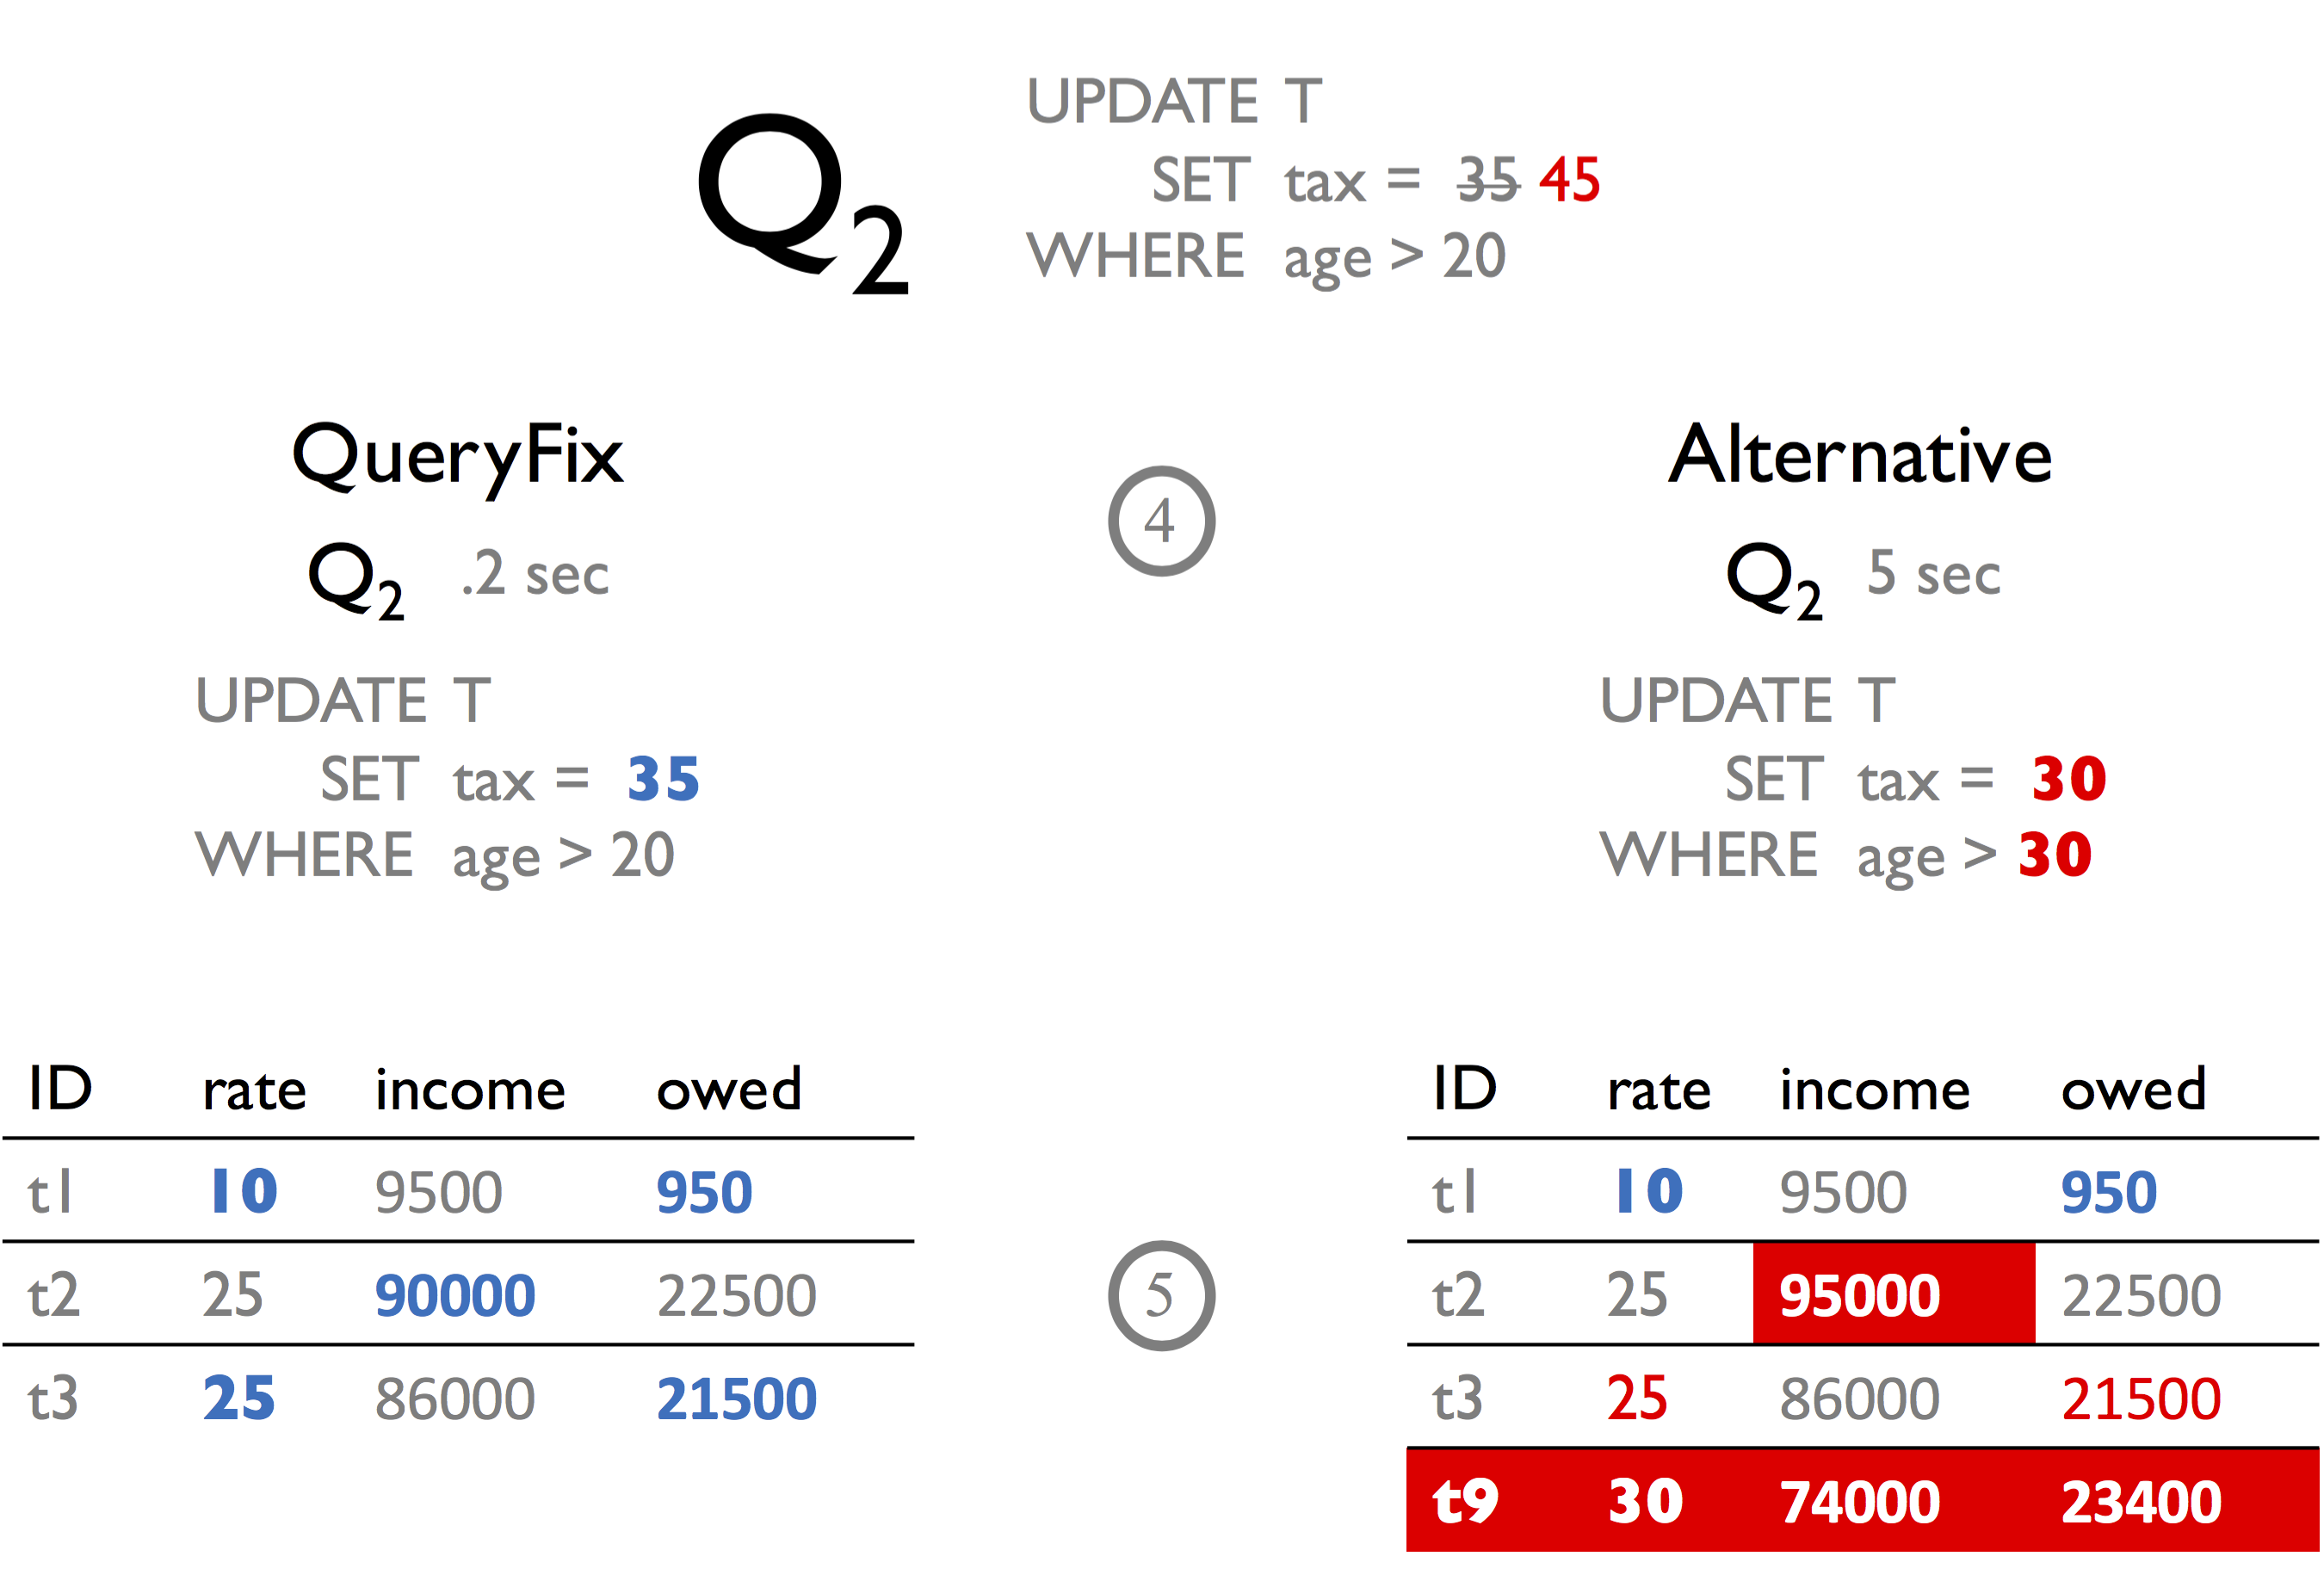
\includegraphics[width = .85\columnwidth]{figures/demo2}
  \caption{Comparisons between proposed fixes.}
  \label{f:demo2} 
\end{figure}

\noindent {\bf Step 4:}  The result page lists the original query ID and text at the top.  The ID 
is important because some proposed fixes may identify an incorrect query.  Below the original query,
the interface shows each of the proposed fixes as columns.  For example, Figure~\ref{f:demo2} shows 
that both the \sys and alternative fixes identified the correct query $Q_2$, however \sys only took $0.2$ seconds
to run, and correctly fixed $Q_2$, whereas the alternative took $5$ sec and proposed an incorrect fix.

\noindent {\bf Step 5:} The bottom tables show the effects of the fixes on the complaints from
step 3.  Correctly fixed attribute values are highlighted in blue, unfixed errors are shown as red text, while incorrectly
fixed values are highlighted with a red background.  Finally, it is possible for proposed fixes to 
{\it introduce} new errors, which are shown as entire rows that are highlighted with a red background.








%%!TEX root = ../main.tex

\section{Related Work}
\label{s:related}

% data cleaning
\sys tackles the problem of diagnosis and repair in relational query
histories (query logs). It does not aim to correct errors in the data
directly, but rather to find the underlying reason for reported errors
in the queries that operated on the data. This is in contrast to
traditional data cleaning~\cite{rahm00, Raman01, Kalashnikov06,
Fan2008b} which focuses on identifying and correcting data
``in-place.'' Identifying and correcting errors is an important, and
rightfully well-studied problem. Existing literature has supplied a
variety of tools to capture errors originating from data
integration~\cite{Abiteboul99, Batini1986, Rahm2001, ParentS98},
recognizing the same entities in data~\cite{Koudas2006,
GruenheidDS14}, identifying true facts among conflicting
data~\cite{yin2008truth, DN09, ltm2012}, and language support for
cleaning~\cite{Galhardas2000}. All of these techniques are
complimentary to our work. Their goal is to identify which data is
correct and which data is incorrect, but they don't look for the
sources of these errors in the processes or queries that generate and
modify this data. In fact the output of such methods can be used to
augment the complaint sets used by \sys, which focuses on identifying
errors in the queries that produced the data, rather than the data
itself.

%repairs
An aspect of data cleaning focuses on providing repairs for the
identified errors~\cite{ChuIP13}. Tools in this domain have targeted
different methods and interactions for providing fixes, ranging from
functional dependencies~\cite{Fan2008b, ChuIP13} and
rules~\cite{Beskales2010, Cong2007} and functional
dependencies~\cite{Fan2008b, ChuIP13}, to interactive methods that
solicit user feedback~\cite{Yakout, Raman01}. As with the other data
cleaning approaches, all these techniques again operate on the data
directly. In contrast, \sys analyzes errors in the data to diagnose
and repair errors in queries that operated on the data. Thus, \sys
leverages the facts that some data errors are systemic, linked to
erroneous updates. Diagnosing the cause of the errors, will achieve
systematic fixes that will correct all relevant errors, even if they
have not been explicitly identified.

%% Data auditor and Data XRay
Closer to exploring systemic reasons and patterns for errors are
techniques such as Data Auditor~\cite{Golab2008, GolabKKS10} and Data
X-Ray~\cite{wang2015}. Both tools tools identify features, which can
be selected from the tuple attributes, that best summarize or describe
groups of tuples (or specifically errors). While these tools can
generate feature sets or patterns of attributes that characterize
errors, these are not linked to the queries, but are again
characterizations over the data itself. Such techniques can be
tremendously useful if the processes that generate or modify the data
are unknown or black-box computations. In these cases, Data Auditor
and Data X-Ray can provide high-level clues for potential problems in
the data derivation process. However, both approaches are oblivious to
the actual queries that operated on the data, and they do not provide
particular fixes. Ontology-based why-not
explanations~\cite{tenCate2015} is very similar to Data X-Ray, but is
only relevant to absent tuples (deletions), and again does not
consider the query history.



%things about diagnosis and explanations


\cite{Golab2008,GolabKKS10 } 

Studying and explaining
data outcome has been studied in many aspects:
\cite{GebalyAGKS14}
focuses on providing 
explanations to particular data outcome in tables; \cite{wang2015}
provides error diagnosing for general data extraction systems. 


% things  about validating updates before executing/cmmit to database
Related work about validating updates in time: 
\cite{Chen2011} validate correctness of updates before performing the update;


% things for exploring wrong or undetermined query,  why not? 
Related works on deriving desired select query: focus on 
Query by example, \cite{dimitriadou2014explore}  uses machine learning
techniques to explore query that satisfy user interests. 


% things about data provenance and data debugging
\cite{mucslu2013data}



Scorpion explanation uses data to synthesize predicates that explain.

Why not work.

View construction and query by example.

Take a look at temporal databases, the CIDR/arxiv paper has a few good starting points. Aditya also dug these out a while back


The way we return results is more like online aggregation or anytime algorithms -- 
as you run longer, the suggested fixes improve because we examine more of the query log.

\url{http://citeseerx.ist.psu.edu/viewdoc/download?doi=10.1.1.49.3765&rep=rep1&type=pdf}

\url{http://people.cs.aau.dk/~csj/Thesis/pdf/chapter26.pdf}


\balance


{
% If you want to use smaller typesetting for the reference list,
% uncomment the following line:
\small
%\bibliographystyle{acm-sigchi}
\bibliographystyle{abbrv}
\bibliography{main}
}

%\techreport{
\appendix

\section{A Learning-based Approach}
\label{sec:heuristic}
  
A drawback of the MILP approach is that the generated models grow with the 
size of the database and query log.
However, we argue that the encoded information is necessary in order to generate a sufficient set of constraints that result in a good repair.
In this section, we examine an alternative, simpler, decision tree-based approach called \dt. 
We show that even in a simple case of a single query log and a complete complaint set, it is expected to perform poorly.
We will first describe how to model the repair process using a decision tree,
and then we will present and discuss experimental results that illustrate its limitations.

\subsection{Modeling Repairs with Decision Trees}

Rule-based learners are used in classification tasks to generate a set of rules, or conjunctive predicates that best classify a group of labeled tuples.
The rules are non-overlapping, and each is associated with a label---a tuple that matches a given rule is assigned the corresponding label.
These rules exhibit a natural parallel with SQL \texttt{WHERE} clauses, 
which can be viewed as labeling selected tuples with a positive label and rejected tuples with a negative label.
Similarly, the structure of the rules is identical to those that \sys is designed to repair.
Thus, given the database tuples labeled to describe the errors, we may use a rule-based learner to
generate the most appropriate \texttt{WHERE} clause.
We focus our attention on rule-based learners;
specifically, we experiment with the C4.5~\cite{quinlan1987} decision tree learner, which is an 
exemplar of rule-based learners.

A core limitation of this classification-based approach is that there is no means to 
repair \texttt{SET} clauses, which modify data values rather than simply label them.
We resolve this with a two step approach.
We first use the decision tree to generate a repair for the
\texttt{WHERE} clause, and then use the modified query to identify repairs for the \texttt{SET} clause.
The need for this two step procedure limits this approach to encoding and repairing at most one query
at a time.

\noindent
\textbf{Repairing the WHERE Clause:}
The \texttt{WHERE} clause of an update query is equivalent to a
rule-based binary classifier that splits tuples into two groups:
(1)~tuples that satisfy the conditions in the \texttt{WHERE} clause
and (2)~tuples that do not. A mistake in a query predicate can 
cause a subset of the tuples to be misclassified, and in turn,
translate into data errors. 
Therefore, repairing the complaints corresponds to repairing the imprecise classification. 

The repair works as follows: For an incorrect query $q$, let
$D_0$ be the database state before $q$, and $D_1^*$ the \emph{correct}
database state that should have been the result after $q$, if $q$ were correct.
We use each tuple $t \in D_0$ as an element in the input training data
for the classifier where the values (of each attribute) of $t$ define
the feature vector and the label for $t$:
	\[
    label(t)= 
    \begin{cases}
    true & \textrm{if\ }D_0.t \neq D_1^*.t\\
    false              & \text{otherwise}
    \end{cases}
\]
The \texttt{true} rules generated by the decision tree trained on this labeled dataset 
forms a disjunction of rules that constitute the repaired \texttt{WHERE} clause.


\noindent
\textbf{Repairing the SET Clause:}
The \texttt{WHERE} clause repair proposed by the classifier may not completely repair 
the complaints if there was also an error in the \texttt{SET} clause. 
In this case, we execute a second repair step.
\begin{figure}[htb]
\centering
  \begin{subfigure} [t]{.75\columnwidth}
  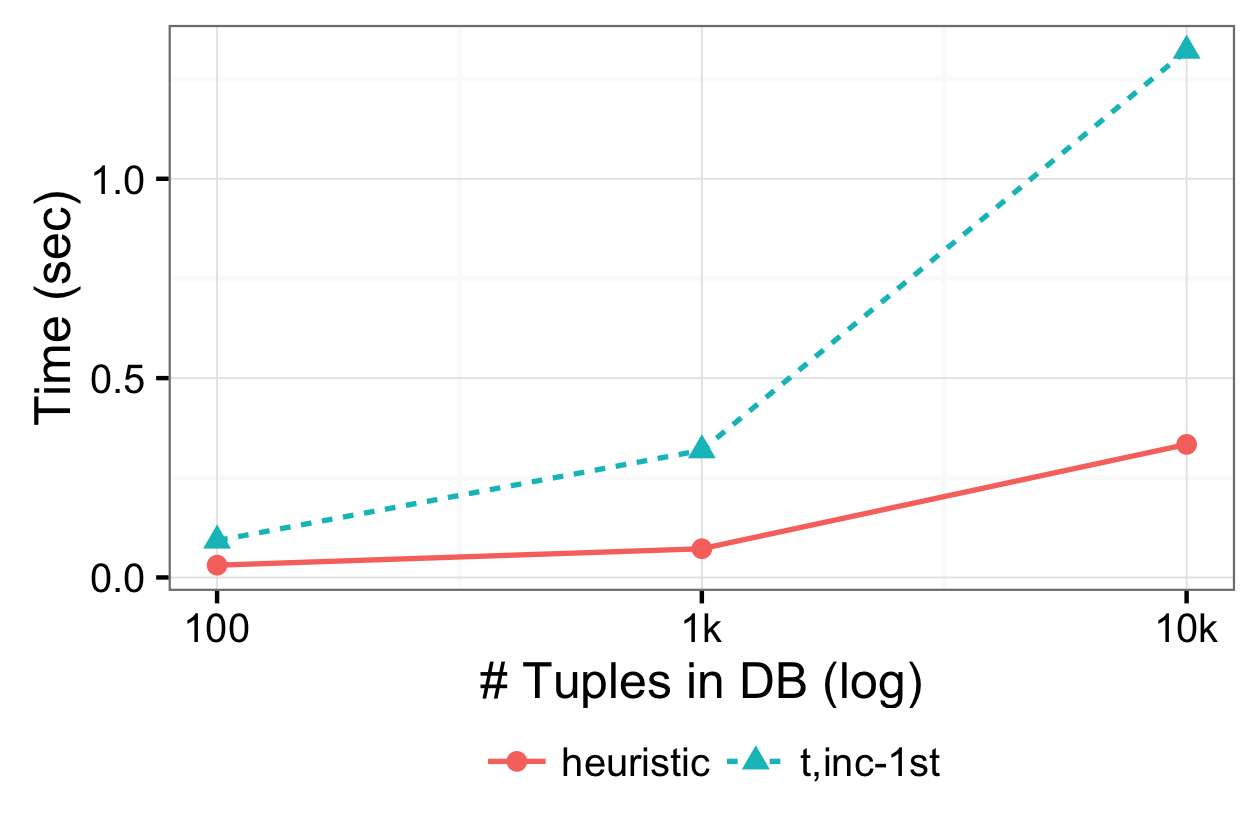
\includegraphics[width = \columnwidth]{figures/heuristictime}
  \caption{Comparison on Performance.}
  \label{f:heuristic_time} 
  \end{subfigure}\\

  \begin{subfigure} [t]{.75\columnwidth}
  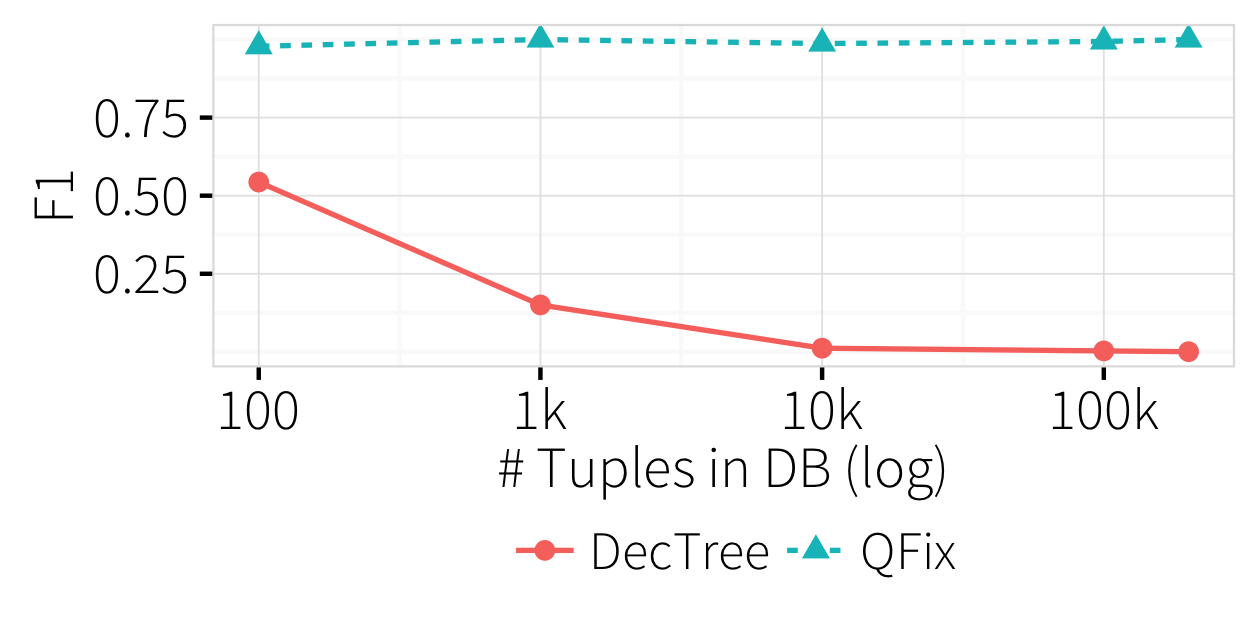
\includegraphics[width = \columnwidth]{figures/heuristicacc}
  \caption{Comparison on Accuracy.}
  \label{f:heuristic_acc} 
  \end{subfigure}
 \caption{\dt compared with \sys}
 \label{f:heuristic}
\end{figure}

We model the errors as a simple linear system of equations: 
each expression in the \texttt{SET} clause is translated into a
linear equation in the same fashion as described in Section~\ref{sec:sol}.
Directly solving the system of equations for the undetermined variables 
will generate the desired repair for the \texttt{SET} expression.



\subsection{Experimental Results}

To illustrate these shortcomings, we compare \dt with \sys using a simplified version of the setup from Section~\ref{sec:experiments} that favors \dt.
We restrict the query log to contain a single query that is corrupted, use a complete complaint set  and vary the database size.
We use the following query template, where all \texttt{SET} clauses assign the attributes to constants,
and the \texttt{WHERE} clauses consist of range predicates:

{\scriptsize
\begin{verbatim}
  UPDATE table
  SET  (a_i=?), ...
  WHERE a_j in [?,?+r] AND ...
\end{verbatim}
}

Figure~\ref{f:heuristic_time} shows that although the runtime performance of \dt is better than \sys by small a constant factor ($\sim 2.5 \times$),
both runtimes degrade exponentially.
In addition, the \dt repairs are effectively unusable as their accuracy is low: the F1-score starts at $0.5$ and rapidly degrades towards $0$.
From these empirical results, we find that \dt generates low-quality repairs even under the simplest conditions---an approach
that applies \dt over more queries is expected to have little hope of succeeding.



There are three important reasons why \dt, and any approach that focuses on a single query at a 
time\footnote{Although our incremental approach tries to generate a repair for a single
query at a time, it encodes all subsequent queries in the log.}, will not perform well.

\iffalse
  \begin{figure*}[t]
  \centering
      \begin{subfigure} [t]{.3\textwidth}
    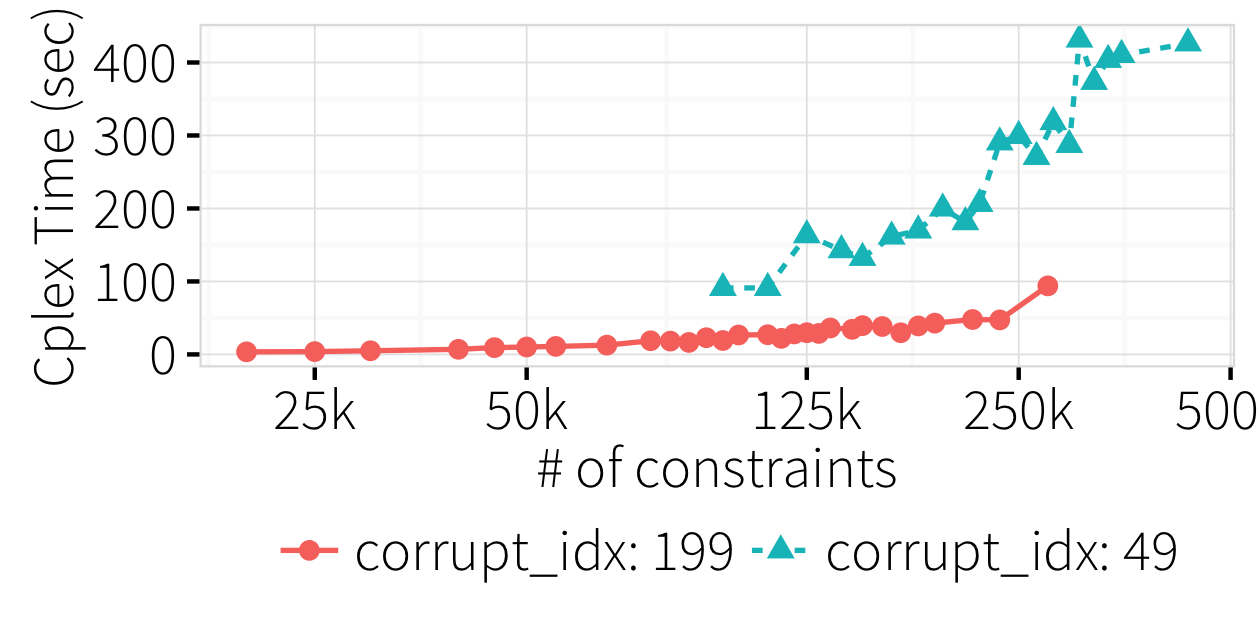
\includegraphics[width = .99\columnwidth]{figures/num_cons_time}
    \vspace*{-.25in}
    \caption{\# of constraints vs. solver solving time.}
    \vspace*{-.1in}
    \label{f:cons_vs_time} 
    \end{subfigure}
    \begin{subfigure} [t]{.3\textwidth}
    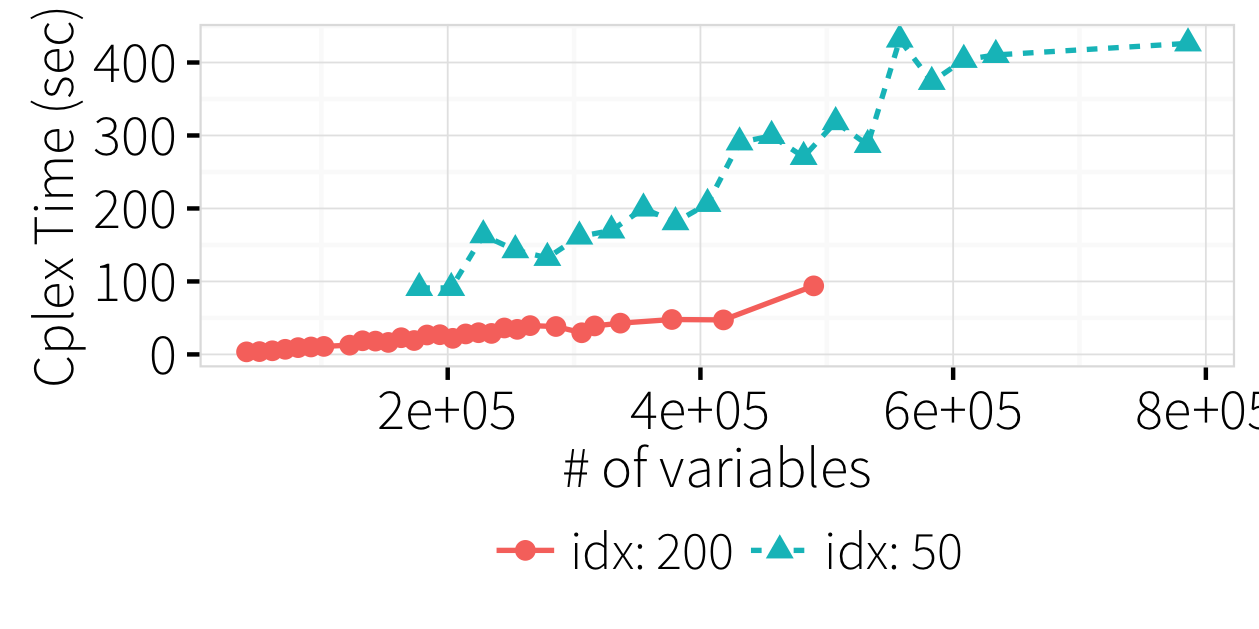
\includegraphics[width = .99\columnwidth]{figures/num_vars_time}
    \vspace*{-.25in}
    \caption{\# of undetermined variables vs. solver solving time.}
    \vspace*{-.1in}
    \label{f:var_vs_time} 
    \end{subfigure}
    \begin{subfigure} [t]{.3\textwidth}
    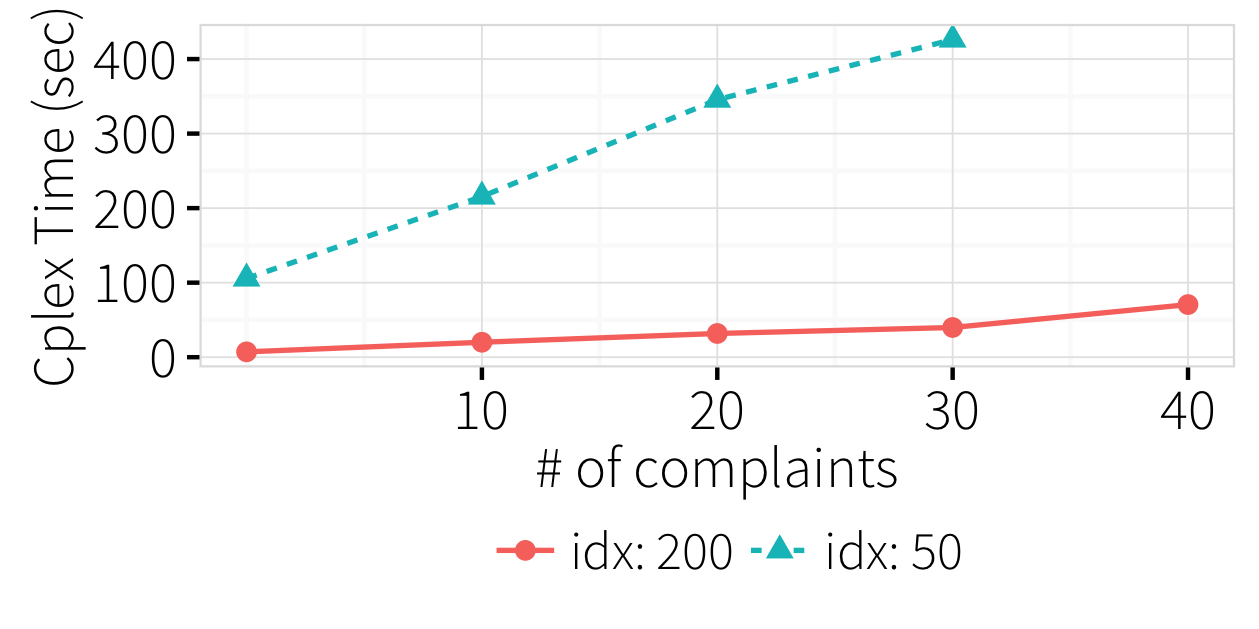
\includegraphics[width = .99\columnwidth]{figures/num_compl_time}
    \vspace*{-.25in}
    \caption{\# of compl. vs. solver solving time.}
    \vspace*{-.1in}
    \label{f:compl_vs_time} 
    \end{subfigure} 
    \iffalse
    \begin{subfigure} [t]{.3\textwidth}
    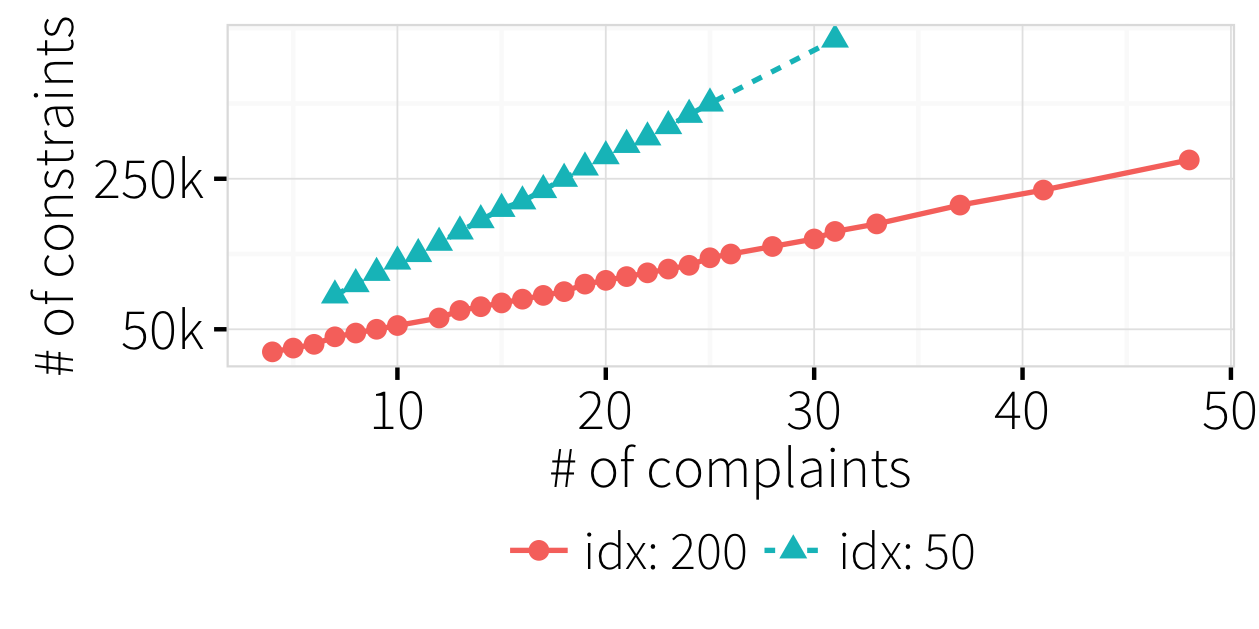
\includegraphics[width = .99\columnwidth]{figures/num_compl_cons}
    \vspace*{-.25in}
    \caption{\# of constraints vs.\# of compl.}
    \vspace*{-.1in}
    \label{f:compl_vs_cons} 
    \end{subfigure}
    \begin{subfigure} [t]{.3\textwidth}
    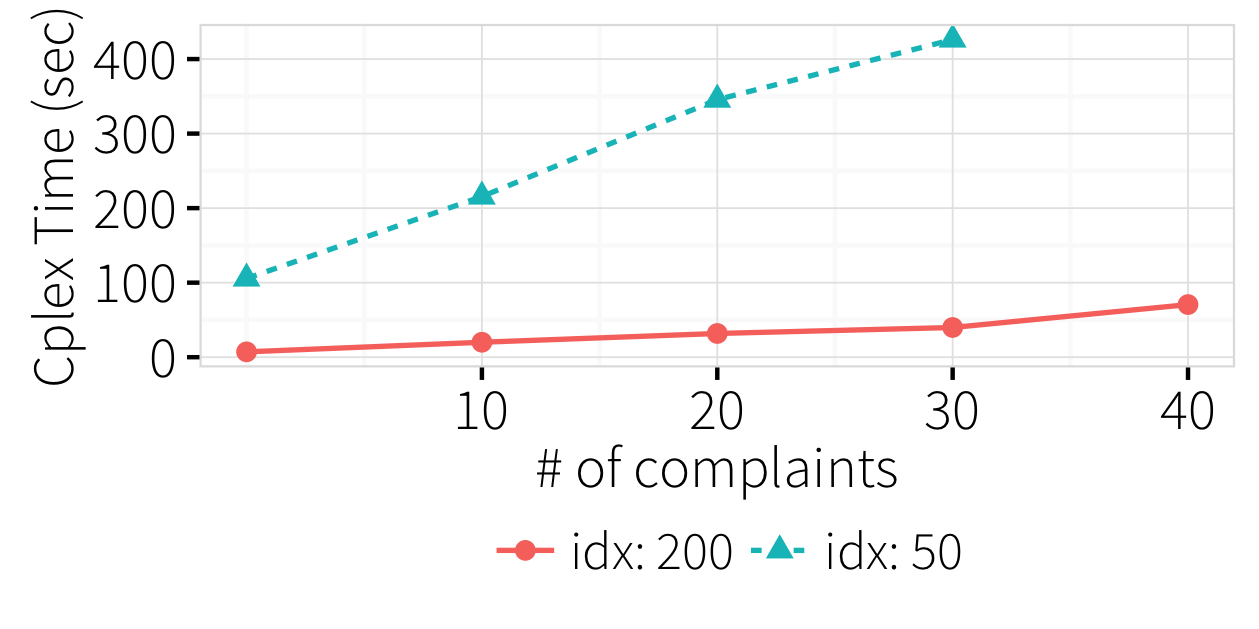
\includegraphics[width = .99\columnwidth]{figures/num_compl_time}
    \vspace*{-.25in}
    \caption{\# of undetermined variables vs. \# of compl.}
    \vspace*{-.1in}
    \label{f:compl_vs_time}
    \end{subfigure}
    \fi
   \caption{Solver solving time grows with all three factors: number of constraints, number of undermined variables and number of complaints. }
   \vspace*{-.1in}
   \label{f:soltime}
  \end{figure*}
\fi
\begin{itemize}[itemsep=1pt, leftmargin=5mm]
\item \textbf{Single Query Limitation: }
In principle, one could attempt to apply this technique to the
entire log one query at a time, starting from the most recent query.
Even ignoring the low repair accuracy shown in Figure~\ref{f:heuristic_acc},
this approach is infeasible.
Consider that we generate a labeled training dataset to repair $q_i$ 
using the query's input and output database states $D_{i-1}$ and $D_i^*$.
Note that $D_i^*$ is the theoretically \emph{correct} database state assuming no errors in the query log.
We would need to derive $D_i^*$ by applying the complaint set to $D_n$ to create $D_n^*$, and roll back the database state.
Unfortunately, \texttt{UPDATE} queries are commonly surjective such
that their inverses are ambiguous, which means that it is often
impossible to derive $D_i^*$. In contrast, the incremental version of
\sys can bypass this problem by encoding subsequent queries in the log
in a MILP representation.


\item \textbf{Structurally Different \texttt{WHERE} Clause Results: } 
The basic classifier approach simply learns a set of rules to minimize
classification error, and can derive a clause whose struture is arbitrarily 
different from the original query's \texttt{WHERE} clause.
Although it may be possible to incorporate a distance measure as part of the decision tree
splitting criteria, it is likely to be a heuristic with no guarantees.


\item \textbf{High Selectivity, Low Precision: }
Classifiers try to avoid overfitting by balancing the complexity of the rules with classification accuracy.
This is problematic for highly selective queries (e.g., primary key updates), because the classifier
may simply ignore the single incorrect record and generate a rule such as \texttt{FALSE}.
In fact, this form of severely imbalanced data continues to be a challenge for most major classification algorithms~\cite{he2009learning, galar2012review}. 
Thus, we believe that alternative classification algorithms would not improve on these results. 
Compound with the fact that many workloads are primarily composed of
key update queries~\cite{oltpbench} this issue severely limits the
applicability of learning-based approaches.

\end{itemize}





\iffalse


\section{MILP Solver Performance}
\label{app:solvtime}

Some background about why we are runnig these experiments.  What is known about MILP solvers already.

\subsection{Factors Relevant to Solver Performance}

\ewu{reference other constraint performance papers}
In this section, we study factors that influence the MILP solver solving time. In this paper, we
use IBM CPLEX~\cite{cplex2014v12} as a black box to solve the constructed MILP problems.  \ewu{describe MILP problems to justify why we focus on num constraints and num variables.} Similar to many solver performance studies~\cite{atamturk2005integer, meindl2012analysis, gearhart2013comparison}, 
we majorly study the connection between solver performance between \textit{the number of constraints} and \textit{the number of variables} in the constructed MILP problem. For this, we create \texttt{UPDATE}-only workloads using our synthetic data generator for 300 queries with constant \texttt{SET} clause and range \texttt{WHERE} clause: 

{\scriptsize
\begin{verbatim}
  UPDATE table
  SET  (a_i=?), ...
  WHERE a_j in [?,?+r] AND ...
\end{verbatim}
}
We further corrupt two query indexes, $q_{50}$ and $q_{200}$, to create the dirty query logs. \xlw{We only show results for  \texttt{UPDATE}-only workloads since all types of workloads show similar correlations. In addition, the selected corrupt query indexes allow us to evaluate the solver performance over median to large problem sizes.}  \ewu{We chose these because...} 


\smallskip
\emph{Number of Constraints: } We first study the relationship between solver performance and number of constraints. \xlw{The number of constraints is controlled via multiple factors including the number of complaints, corrupt query index, complexity of queries. Due to the randomness in synthetic data generator, we are not able to control the size of constraints to a specific value.} \ewu{Explain that the number of constraints is not controlled by you, which is why the lines start and end at different values in the figures.} From Figure~\ref{f:cons_vs_time}, we observe that solver time is roughly positive proportional, with tiny fluctuation, to the number of constraints in both corrupt indexes. This is expected because increasing the number of constraints by large scale usually accompany with significantly greater amount of variables in the MILP problem, which lead to harder MILP problems by natural. However, MILP problems \ewu{cite MILP papers that say this, so it's clear we are describing well known problems} with slightly larger amount of constraints sometimes could be even easier to solve since the additional constraints help pruning the searching space for similar amount of variables.

\smallskip
\emph{Number of Variables: } Similar to the previous experiment, we next compare the solver time with the number of variables. As shown in Figure~\ref{f:var_vs_time}, we find highly correlated trends compare to Figure~\ref{f:cons_vs_time}. 
This is due to the way we construct the MILP problem: the number of constraints and the number of variables grows linearly with \textit{the number of queries and the number complaints}.  



\iffalse
 In our experiments we found that increasing the number of constraints by increasing the database, query log, or complaint set sizes aversely affects the solver performance,
  solver performance has been shown to \emph{improve} as constraints that effectively reduce the problem space are added to the problem.  
  Thus, we now focus on the effects on the number of undetermined variables, which strictly increases the problem space.
  We keep the number of constraints fixed, however increase the number of undetermined variables by \ewu{XL fill in}. \xlw{need to rerun exp to get required numbers. We need to gradually increase the batch size to achieve this. }

\fi

In Figure~\ref{f:compl_vs_time} we illustrate the above argument by comparing the average solver time between the number of complaints at two different corrupt indexes. This allows us to study the relationship between solver time with both the number of complaints (x-axis) and the number of queries (two indexes). As expected, with the same number of complaints, the solver solving time for corrupt index $50$ is significantly higher than index $200$ since the number of queries encoded in each problem is $250$ and $100$ respectively. In contrast, with the same corrupt query index, problems with higher amount of complaints has much higher average solver solving cost than problems with lower amount of complaints. We believe that this is because increasing the number of queries and the number of complaints would increase both the number of variables and constraints in the constructed MILP problem. 

\xlw{The number of variables and constraints are two quantifiable factors that influence the solver time in solving MILP problems. However, there are other non-quantifiable factors, including but not limited to the correlations among variables, searching space of under-determined variables after pre-processing, that also relevant to the hardness of the MILP problem, which determines the solver time. These non-quantifiable factors are hard to control and optimize. Thus, in this paper, we mainly focus on optimizing (reducing) the quantifiable factors -- number of variables and constraints in order to reduce the  solver time. }

\subsection{Factors Relevant to the Number of Complaints}

From the above experiments, we observe that the solver time is highly correlated to the number of complaints and the number of queries we encoded in a MILP problem. The number of queries can be easily controlled by a particular parameter $N_q$. The number of complaints, on the other hand, is a reflection of the queries that have run over the database. It is influenced by  factors including the \texttt{SET} clause type, corrupt query index, query skewness, \texttt{WHERE} clause range, and some random factors. \ewu{however, don't know how the affect the complaint set.}  To better understand factors that control the size of the complaint set, we ran simulations using a database with $20$ attributes, and a query log of size $1000$ containing
either all constant or relative \texttt{SET} clause \texttt{UPDATE} queries. We found that SET and relative queries behave differently.
We varied the number of corrupt index uniformly throughout the query log, and additionally varied
the skew and range parameters to study how they affect the size of the complaint sets.



\begin{figure}[h]
\centering
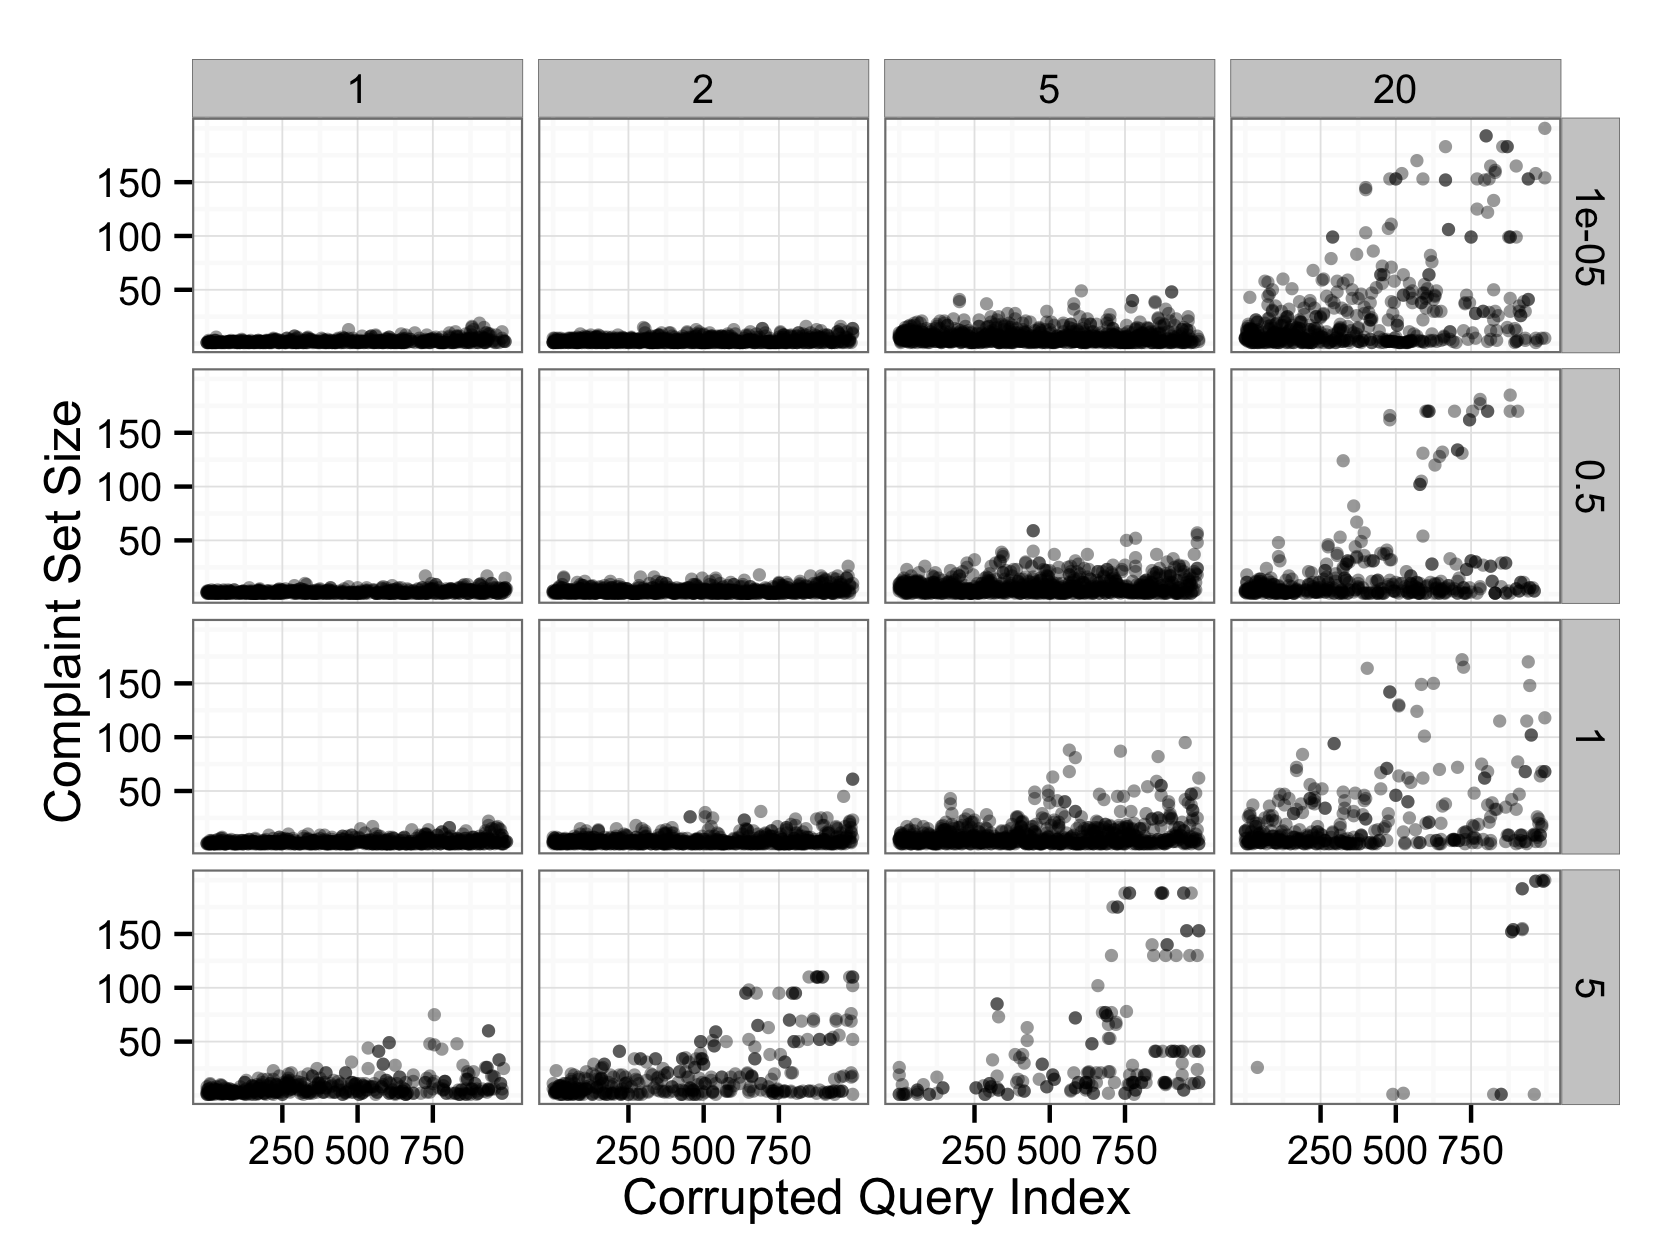
\includegraphics[width = 3in]{figures/qidxsimulation/qidx_v_ncomplaints_20attrs_const}
\caption{Corrupt query index, skew, range vs complaint set size for \textit{constant} \texttt{SET} clauses.}
\label{f:qidx_v_ncomplaints_const} 
\end{figure}

\smallskip
\emph{Constant \texttt{SET} clause: } Figure~\ref{f:qidx_v_ncomplaints_const} plots a representative set of parameters including corrupt query index, range, and skew. We plot one point
for each corrupted query index that results in a complaint set with at least one complaint. 
These results highlight several interesting trends:  With small update range and small skew factor (left upper corner)
the size of the complaint sets are relatively small, and their frequency is constant across the possible query indices.
However as we increase the range and skew, more recent queries are more likely to result in very large complaint sets (at times the size of the database).   
This effect is because the queries that have higher overlap of their \texttt{WHERE} clauses will set groups of tuples to the same value,
and over time, skew the distribution of tuple values to a small number of possible values. 
Thus, more recent corruptions that affect a large cluster of similar tuples will result in a large complaint set.
\ewu{This this effect an artifact of bad experiment design (of our query generation), or is it something that would always happen?  Need to address, since obvious question!}
And the possibility of query overlap increases with update range and skew as these two factors increase the likelihood that queries share the same \texttt{WHERE} and \texttt{SET} clause. 



\begin{figure}[t]
\centering
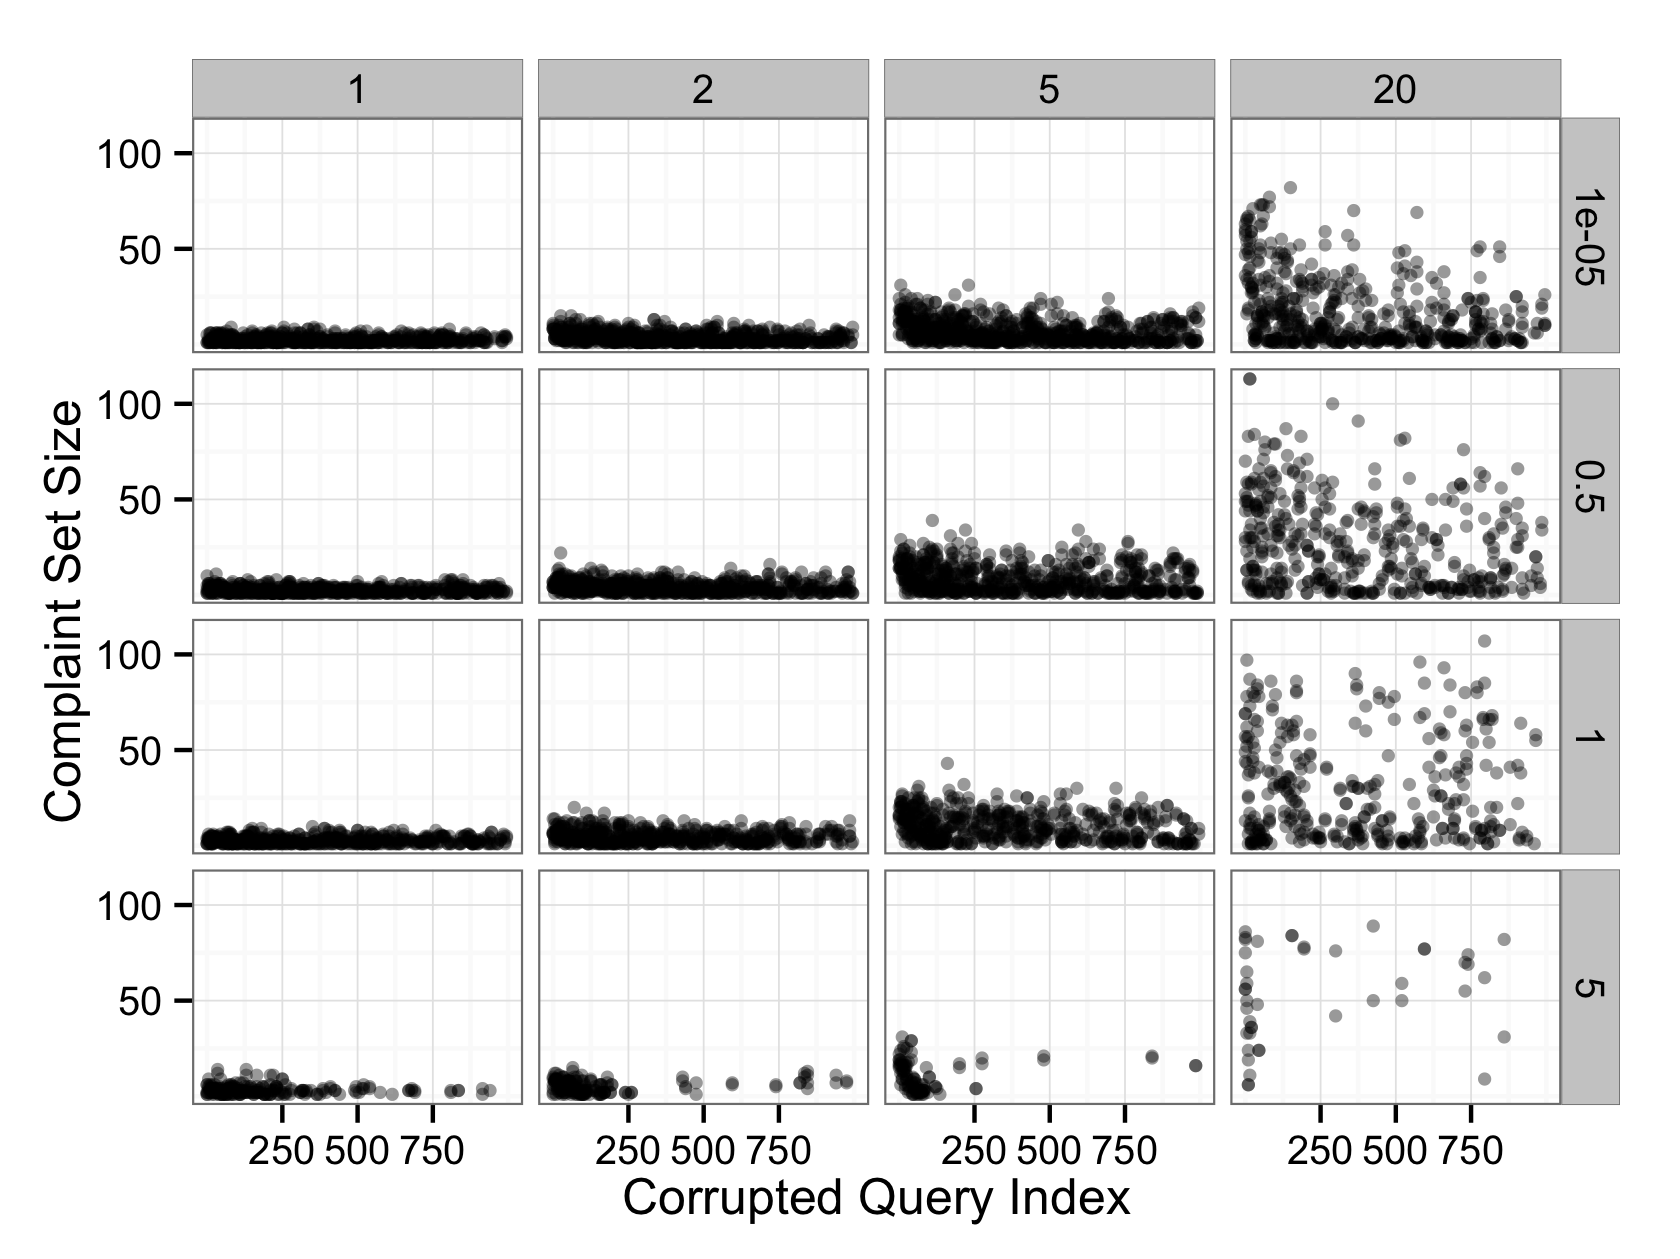
\includegraphics[width = 3in]{figures/qidxsimulation/qidx_v_ncomplaints_20attrs_rel}
\caption{Query index vs complaint set size for $set = rel$.}
\label{f:qidx_v_ncomplaints_rel} 
\end{figure}

\smallskip
\emph{Relative \texttt{SET} clause: } \xlw{In contrast to \textit{constant} \texttt{SET} queries, Figure~\ref{f:qidx_v_ncomplaints_rel} executes the 
same experiment using \textit{relative} \texttt{SET} queries.  In this setting, we find that the trend is
reversed, and older corruptions tend to result in larger complaint sets.  This is because,
subsequent \texttt{UPDATE} queries increment or decrement the attribute value, rather than
overwriting it with a constant value.  The clustering of data values due to query overlap
then increases the number of other tuples affected.
}



\begin{figure*}[ht]
	{\scriptsize
    \begin{minipage}[t]{0.2\textwidth}
         \vspace{0pt} 
         \centering
        \begin{tabular}{lllll}
            \multicolumn{5}{l}{\emph{table}: $D_0$}\\
            \toprule
            \textbf{ID}  & \textbf{$a_1$}    & \textbf{$a_2$} & \textbf{$a_3$} & \textbf{$a_4$} \\
            \midrule
            0 & 8 & 4 & 12 & 28\\
            1 & 2 & 10 & 15 & 3\\
            \bottomrule
            \\
    \end{tabular}
    \end{minipage}
     \begin{minipage}[t]{0.5\textwidth}
         \vspace{0pt} 
         \centering
        \begin{tabular}{l}
            \multicolumn{1}{l}{A \texttt{DELETE} workload  $\mathcal{Q}_{del}$:                                                            }\\
             \toprule
            \texttt{Q1: DELETE FROM table WHERE $a_2$ in \sout{[3,5]} {\color{red}[30, 50]}} \\
   			\texttt{Q2: DELETE FROM table WHERE $a_3$ in [7, 8] }\\ \hline
    \end{tabular}
    \end{minipage}
    \begin{minipage}[t]{0.2\textwidth}
         \vspace{0pt} 
         \centering
       \begin{tabular}{lllll}
            \multicolumn{5}{l}{\emph{table}: $D_1$ after execute $\mathcal{Q}_{del}$}\\
            \toprule
            \textbf{ID}  & \textbf{$a_1$}    & \textbf{$a_2$} & \textbf{$a_3$} & \textbf{$a_4$} \\
            \midrule
            \rowcolor{mid-gray}
            \sout{0} & \sout{8} & \sout{4} & \sout{12} & \sout{28}\\
            1 & 2 & 10 & 15 & 3\\
            \bottomrule
            \\
\end{tabular}
    \end{minipage} \\
  \begin{minipage}[t]{0.2\textwidth}
         \vspace{0pt} 
         \centering
        \begin{tabular}{lllll}
        
            
    \end{tabular}
    \end{minipage}
 \begin{minipage}[t]{0.5\textwidth}
         \vspace{0pt} 
         \centering
        \begin{tabular}{l}
   			\multicolumn{1}{l}{A \texttt{UPDATE} workload $\mathcal{Q}_{up}$:                              }\\
   			 \toprule
            \texttt{Q1: UPDATE table SET $a_1$ = 10 WHERE $a_2$ in \sout{[3,5]} {\color{red}[30, 50]}} \\
   			\texttt{Q2: UPDATE table SET $a_4$ = 7 WHERE $a_3$ in [7, 8] }\\ \hline
            \\
    \end{tabular}
    \end{minipage}     
    \begin{minipage}[t]{0.2\textwidth}
         \vspace{0pt} 
         \centering
\begin{tabular}{lllll}
            \multicolumn{5}{l}{\emph{table}: $D_1'$ after execute $\mathcal{Q}_{up}$}\\
            \toprule
            \textbf{ID}  & \textbf{$a_1$}    & \textbf{$a_2$} & \textbf{$a_3$} & \textbf{$a_4$} \\
            \midrule
            \rowcolor{mid-gray}
            0 & \color{red}{8} & 4 & 12 & 28\\
            1 & 2 & 10 & 15 & 3\\
            \bottomrule
            \\
\end{tabular}
    \end{minipage}
}
    \vspace{-2mm}
    \caption{A initial database state $D_0$ and database states after apply $\mathcal{Q}_{del}$ and $\mathcal{Q}_{up}$ on $D_0$. }
    \label{fig:example2}
\end{figure*}
\section{Repairing the Correct Query}
\label{app:index}

The experimental section (Section~\ref{sec:experiments}) primarily focused on performance and accuracy measures of the repairs, and for space constraints, ignored 
whether the proposed repair was actually the correct query (it is possible we fix an incorrect query in a way that resolves the complaint set).
Although we found in most circumstances we identify the correct query to fix, we now turn our attention to better understand 
the conditions when we may fix the incorrect query. 

   \begin{figure*}[t]
  \centering
  \begin{subfigure} [t]{.3\textwidth}
    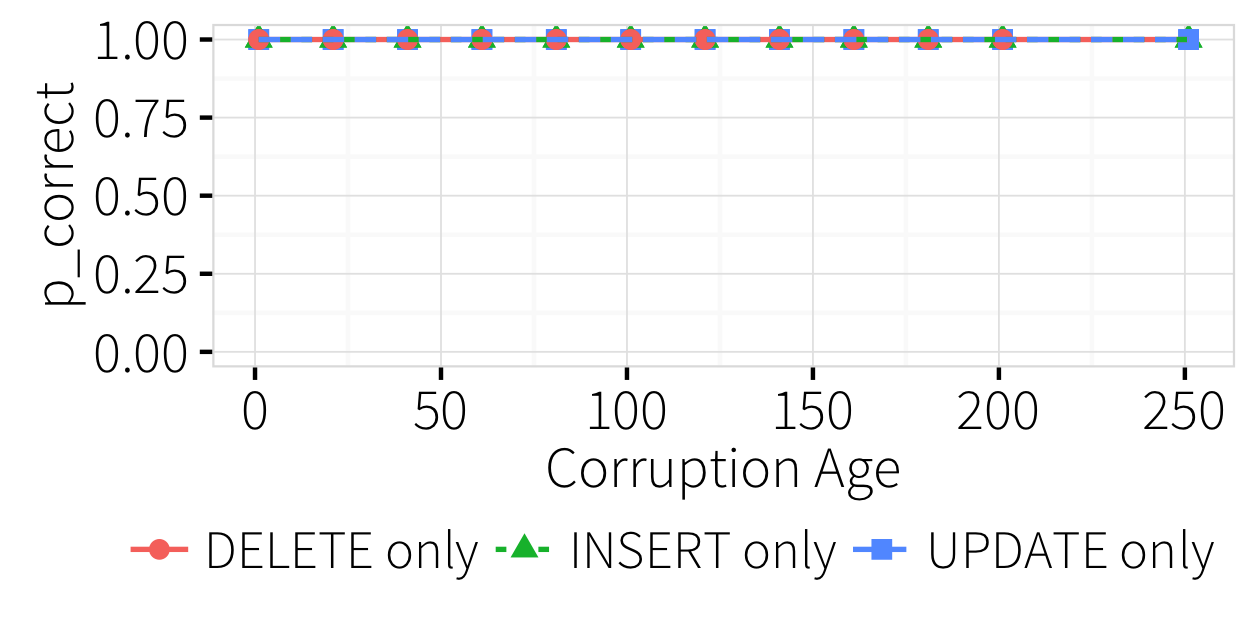
\includegraphics[width = .99\columnwidth]{figures/indelup_acc_idx}
    \vspace*{-.25in}
    \caption{Correct repair ratio vs. query types}
    \label{f:querytyperatio} 
    \end{subfigure}
    \begin{subfigure} [t]{.3\textwidth}
    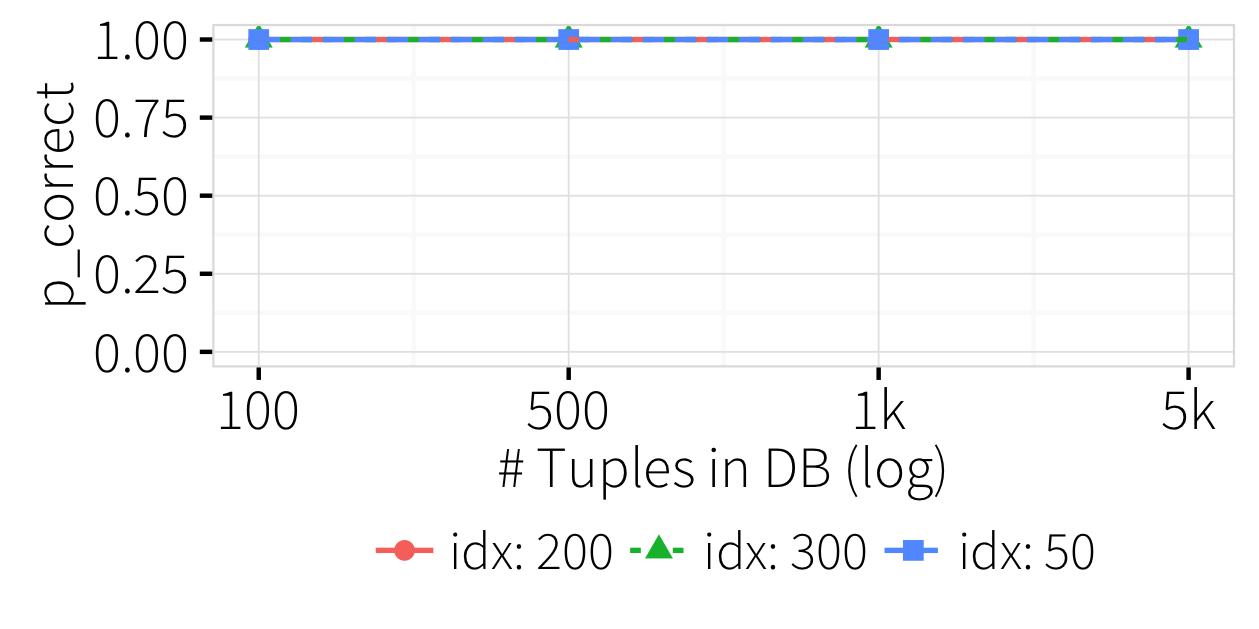
\includegraphics[width = .99\columnwidth]{figures/dbsize_acc_idx}
    \vspace*{-.25in}
    \caption{Correct repair ratio vs. database sizes}
    \label{f:dbsizeratio} 
    \end{subfigure}
    \begin{subfigure} [t]{.3\textwidth}
    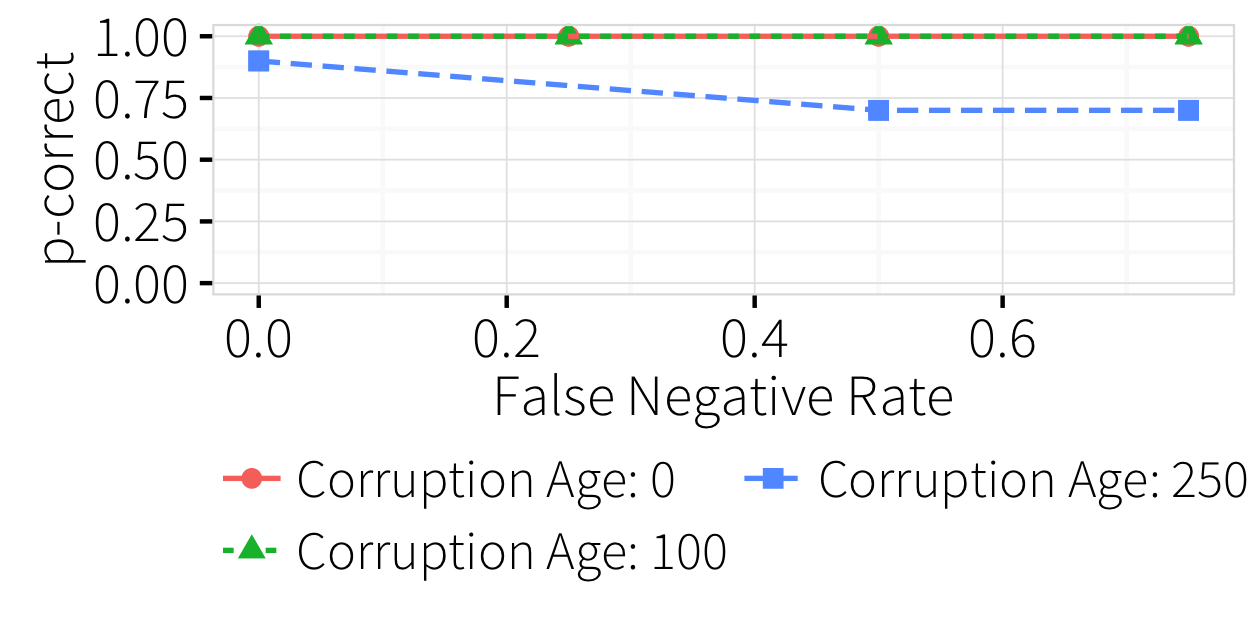
\includegraphics[width = .99\columnwidth]{figures/noise_fn_acc_idx}
    \vspace*{-.25in}
    \caption{Correct repair ratio vs. false negatives}
    \label{f:fnratio} 
    \end{subfigure} \\
    \begin{subfigure} [t]{.3\textwidth}
    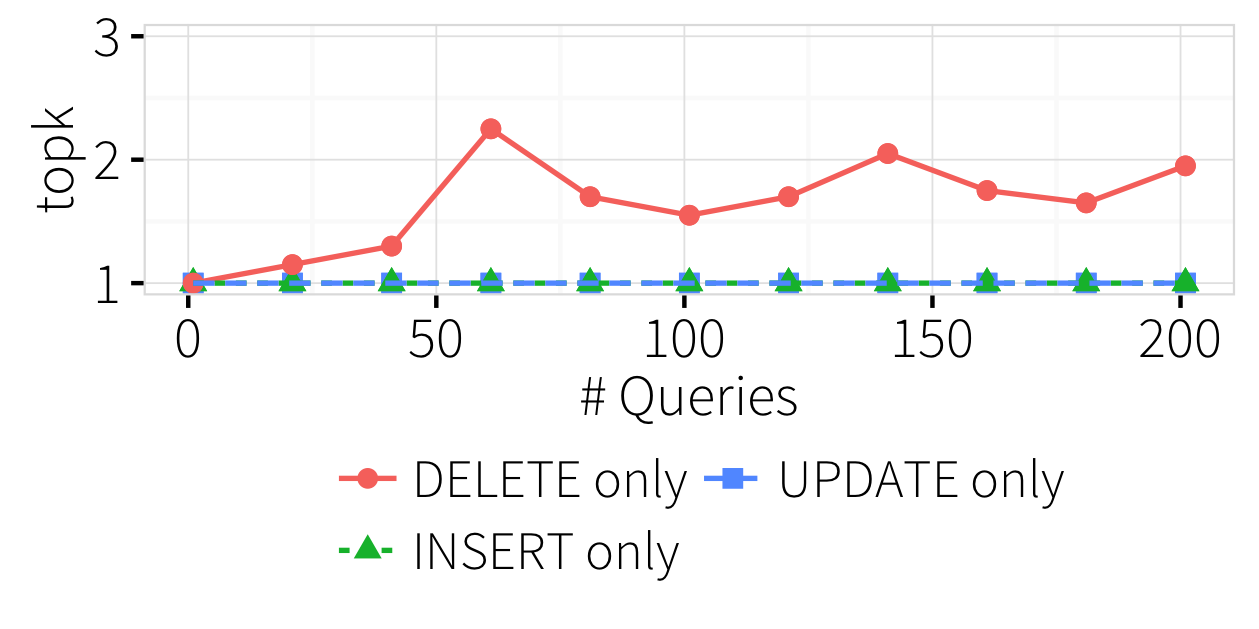
\includegraphics[width = .99\columnwidth]{figures/indelup_fixcount}
    \vspace*{-.25in}
    \caption{Top-k vs. query types. }
    \vspace*{-.1in}
    \label{f:querytypefixcount} 
    \end{subfigure}
    \begin{subfigure} [t]{.3\textwidth}
    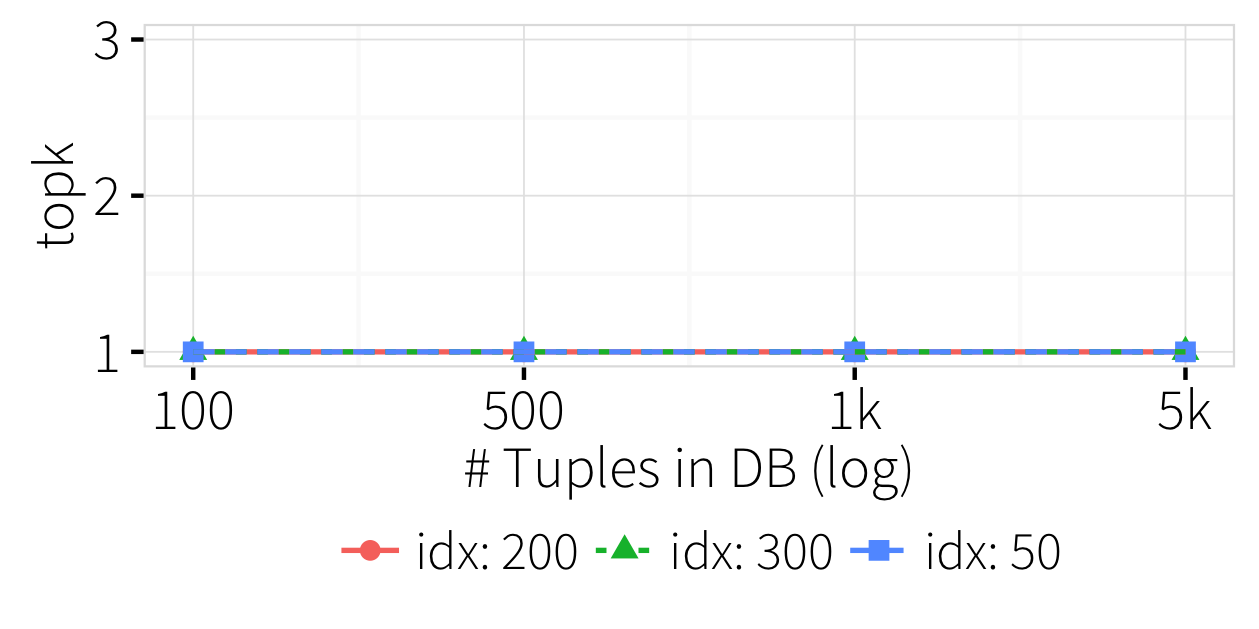
\includegraphics[width = .99\columnwidth]{figures/dbsize_fixcount}
    \vspace*{-.25in}
    \caption{Top-k vs. database sizes. }
    \vspace*{-.1in}
    \label{f:dbsizecount} 
    \end{subfigure}
    \begin{subfigure} [t]{.3\textwidth}
    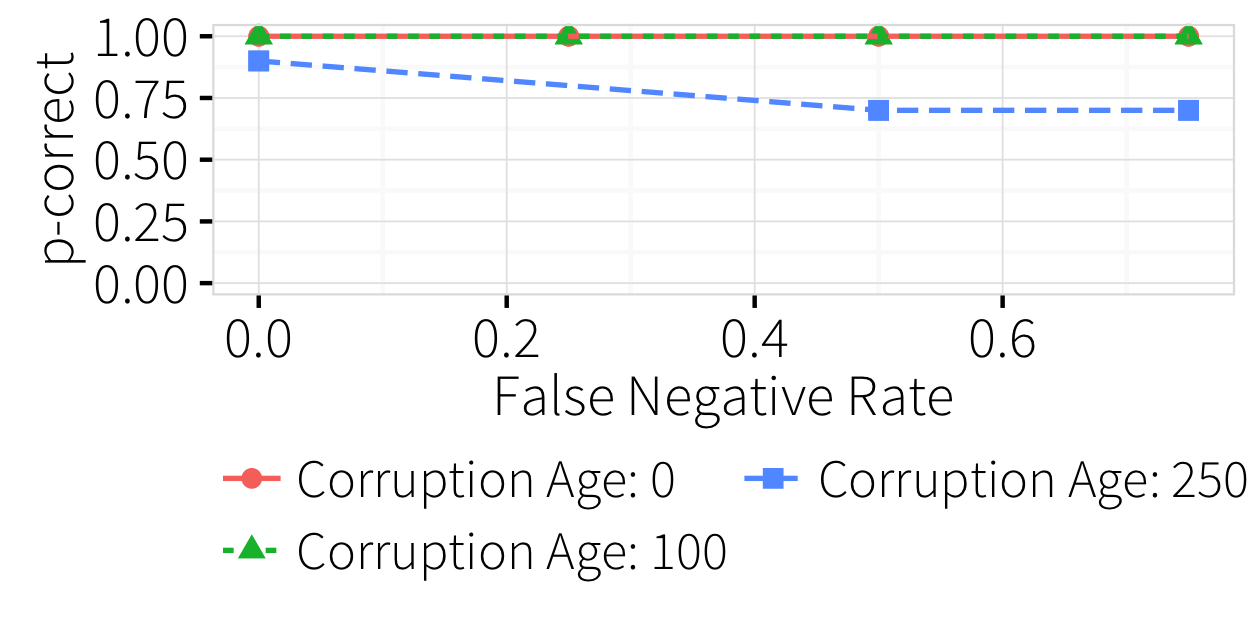
\includegraphics[width = .99\columnwidth]{figures/noise_fn_acc_idx}
    \vspace*{-.25in}
    \caption{Top-k vs. false negatives (\color{red}{not complete!})}
    \vspace*{-.1in}
    \label{f:fnfixcount} 
    \end{subfigure}
   \caption{Correct repair ratio and number of candidate fixes of \sys varies on different types of workloads and false negative rate but remain 
   stable for with increasing number of tuples on \texttt{UPDATE} workload.}
   \vspace*{-.1in}
   \label{fig:truerate}
  \end{figure*}


\subsection{Experimental Results}
To evaluate \sys's ability in identifying the correct query to fix, we execute QFix over 20 random runs and summarize our results using two evaluation metrics:
The first $p_{correct}$ computes the ratio between the number of runs where \sys correctly repairs the corrupt query and where \sys
repairs the wrong query; The second metric $topk$ measures the number of repairs that \sys proposes before repairing the true corrupt query.
The second metric is useful to quantify the extent that \sys's repairs are false positives (though they may correctly resolve the complaint set).
A small $topk$ value suggests that \sys is still effective at providing repair \emph{recommendations} as part of a diagnostic interface.

\textbf{Correct repair ratio vs. query types: } In Figure~\ref{f:querytyperatio}, we first evaluate $p_{correct}$ rate on three types of workloads: \sys identifies the correct query to fix ($p_{correct} = 1.0$ and $topk = 1$) for \texttt{UPDATE} and \texttt{INSERT} workloads but unstable and much lower rate for \texttt{DELETE} workload. This is expected since more information of the actual incorrectness get maintained through \texttt{UPDATE} queries by the updated tuple values. \ewu{Is this because the problem is fundamentally underconstrained?  if so, explain in those terms and describe why.} However, such information get lost and obscured for \texttt{DELETE} queries as those deleted tuples no longer exist in the database. As a result, actual incorrect queries in \texttt{UPDATE} workloads are much easier to identify than those in \texttt{DELETE} workloads. \texttt{INSERT} workloads are easy to fix by natural since each \texttt{INSERT} query only touches one tuple. 

To further illustrate this, we present the following toy example (Figure~\ref{fig:example2}) of two simple query logs, one for \texttt{DELETE} workload and one for \texttt{UPDATE} workload, that operate on the same initial database state and with the exact same \texttt{WHERE} clauses. 

In the above example, we find that there exist two candidate fixes for the \texttt{DELETE} workload $\mathcal{Q}_{del}$: one can either modify the \texttt{WHERE} clause of $Q2$ to $[12, 12]$ or the \texttt{WHERE} clause of $Q1$ to $[4, 4]$. In addition, the two candidate fixes achieve the exact same final database state. However, there only exists one candidate fix for the \texttt{UPDATE} workload $\mathcal{Q}_{up}$ since values in every attribute must satisfy with the desired database state. According to the converted constraints, modifying $Q2$ cannot solve the problem since it would not fix the value in the incorrect attribute $a_1$.  

\textbf{Top-k vs. query types: } In Figure~\ref{f:querytypefixcount}, we observe the same trend: the $topk$ count for \texttt{UPDATE} and \texttt{INSERT} workloads remain $1$ across all query indexes while the $topk$ count shows unstable and much higher value for \texttt{DELETE} workloads. Overall, we find \sys above is able to find the true repair within 3 diagnosis over more than 85\% of all random runs. 

\textbf{Correct repair ratio \& top-k vs. database sizes: } We next narrow down to \texttt{UPDATE} workload and evaluate \sys's behavior with increasing amount of tuples in the database. We observe $p_{correct} = 1$ and $topk = 1$ on different corrupt indexes in all database sizes (Figure~\ref{f:dbsizeratio}~\ref{f:dbsizecount}). 

\textbf{Correct repair ratio \& top-k vs. false negatives: } We finally evaluate \sys on \texttt{UPDATE} workload with increasing false negative rates. Similar to the quality drop in Figure~\ref{f:falsenegative_acc}, we observe the $p_{correct}$ (Figure~\ref{f:fnratio}) rate also suffers from less submitted complaints when errors happen early in the query log. However, \sys achieves above $0.75$ $p_{correct}$ rate for more recent errors (corrupt index is 300 and 200) even with high false negative rate. The $topk$ behaves similar to $p_{correct}$ in which $topk$ increasing with the false negative rate (Figure~\ref{f:fnfixcount}).  
\fi}






\end{document}
